% =============================================================================
%  main.tex
%  Governing Generative Landscape Design: A Formal Mathematical Framework
%  for 4D Gaussian Splatting and Semantic Hypergraph Integration in
%  Indigenous Heritage Reconstruction
%
%  Authors : Alejandro Soto Franco, Hamza Woodson
%  Engine  : XeLaTeX  (xelatex main && biber main && xelatex main x2)
% =============================================================================
\documentclass[11pt,a4paper]{article}

% ── Mathematics ──────────────────────────────────────────────────────────────
\usepackage{amsmath,amssymb,amsthm,mathtools}

% ── Typography (XeLaTeX) ─────────────────────────────────────────────────────
\usepackage{fontspec}
\setmainfont{Latin Modern Roman}
\usepackage{microtype}

% ── Page geometry ────────────────────────────────────────────────────────────
\usepackage[
    a4paper,
    top    = 25mm,
    bottom = 30mm,
    left   = 25mm,
    right  = 25mm,
]{geometry}
\usepackage{setspace}
\setstretch{1.08}

% ── Figures and tables ───────────────────────────────────────────────────────
\usepackage{graphicx}
\usepackage{subcaption}
\usepackage{booktabs}
\usepackage{array}
\usepackage{tabularx}
\usepackage{multirow}
\usepackage{float}

% ── TikZ ─────────────────────────────────────────────────────────────────────
\usepackage{tikz}
\usetikzlibrary{
    shapes.geometric,
    arrows.meta,
    positioning,
    calc,
    fit,
    backgrounds,
    decorations.pathreplacing,
    decorations.markings,
}

% ── Colours and hyperlinks ───────────────────────────────────────────────────
\usepackage{xcolor}
\definecolor{linkblue}{HTML}{1D4ED8}
\definecolor{eqred}{HTML}{B91C1C}
\definecolor{spatialblue}{HTML}{DBEAFE}
\definecolor{semanticgreen}{HTML}{D1FAE5}
\definecolor{fusionamber}{HTML}{FEF3C7}
\definecolor{genrose}{HTML}{FCE7F3}
\definecolor{darkblue}{HTML}{1E3A8A}
\definecolor{darkgreen}{HTML}{064E3B}
\definecolor{darkteal}{HTML}{0F4C81}
\definecolor{nodestr}{HTML}{3B82F6}
\definecolor{nodeact}{HTML}{10B981}
\definecolor{nodenar}{HTML}{F59E0B}
\definecolor{noderul}{HTML}{EF4444}
\definecolor{nodeevt}{HTML}{8B5CF6}
\usepackage[
    colorlinks  = true,
    linkcolor   = linkblue,
    citecolor   = linkblue,
    urlcolor    = linkblue,
    pdfauthor   = {Alejandro Soto Franco and Hamza Woodson},
    pdftitle    = {Governing Generative Landscape Design},
]{hyperref}
\usepackage{cleveref}

% Red equation cross-references
\let\oldeqref\eqref
\renewcommand{\eqref}[1]{%
    \hyperref[#1]{\textcolor{eqred}{(\ref*{#1})}}%
}

% ── Lists ────────────────────────────────────────────────────────────────────
\usepackage{enumitem}

% ── Coloured boxes ───────────────────────────────────────────────────────────
\usepackage{tcolorbox}
\tcbuselibrary{skins,breakable}

\newtcolorbox{insightbox}[1][]{
  enhanced, breakable,
  colback  = linkblue!6,
  colframe = linkblue!60,
  fonttitle= \bfseries,
  title    = {Key insight},
  #1
}
\newtcolorbox{constructbox}[1][]{
  enhanced, breakable,
  colback  = darkgreen!5,
  colframe = darkgreen!50,
  fonttitle= \bfseries,
  title    = {Construction},
  #1
}

% ── Bibliography ─────────────────────────────────────────────────────────────
\usepackage[
    style      = numeric-comp,
    sorting    = none,
    backend    = biber,
    maxbibnames= 6,
]{biblatex}
\addbibresource{references.bib}

% ── Theorem environments ─────────────────────────────────────────────────────
\theoremstyle{plain}
\newtheorem{theorem}{Theorem}[section]
\newtheorem{proposition}[theorem]{Proposition}
\newtheorem{lemma}[theorem]{Lemma}
\newtheorem{corollary}[theorem]{Corollary}

\theoremstyle{definition}
\newtheorem{definition}[theorem]{Definition}
\newtheorem{assumption}[theorem]{Assumption}

\theoremstyle{remark}
\newtheorem{remark}[theorem]{Remark}
\newtheorem{example}[theorem]{Example}

% ── Notation macros ──────────────────────────────────────────────────────────

% Calculus
\newcommand{\dd}{\mathrm{d}}
\newcommand{\pfrac}[2]{\frac{\partial #1}{\partial #2}}

% Linear algebra
\newcommand{\mbf}[1]{\mathbf{#1}}
\newcommand{\abs}[1]{\left\lvert #1 \right\rvert}
\newcommand{\norm}[1]{\left\lVert #1 \right\rVert}
\newcommand{\vech}{\operatorname{vech}}
\newcommand{\tr}{\operatorname{tr}}
\newcommand{\diag}{\operatorname{diag}}

% Probability / statistics
\newcommand{\E}{\mathbb{E}}
\newcommand{\Var}{\operatorname{Var}}
\DeclareMathOperator*{\argmin}{arg\,min}
\DeclareMathOperator*{\argmax}{arg\,max}

% Lie groups
\newcommand{\SO}{\mathrm{SO}}
\newcommand{\SE}{\mathrm{SE}}
\newcommand{\so}{\mathfrak{so}}

% Gaussian scene
\newcommand{\GS}{\mathcal{G}}

% Hypergraph components
\newcommand{\HG}{\mathcal{H}}
\newcommand{\Struc}{\mathcal{S}}
\newcommand{\Act}{\mathcal{A}}
\newcommand{\Nar}{\mathcal{N}}
\newcommand{\Rul}{\mathcal{R}}
\newcommand{\Evt}{\mathcal{V}}
\newcommand{\Tv}{\mathcal{T}_V}
\newcommand{\Te}{\mathcal{T}_E}

% Alignment and embedding
\newcommand{\inst}{\psi}
\newcommand{\gvec}{\mathbf{g}}
\newcommand{\hvec}{\mathbf{h}}
\newcommand{\zvec}{\mathbf{z}}

% Loss functions
\newcommand{\Lrec}{\mathcal{L}_{\mathrm{recon}}}
\newcommand{\Lstruct}{\mathcal{L}_{\mathrm{struct}}}
\newcommand{\Lgov}{\mathcal{L}_{\mathrm{gov}}}
\newcommand{\Ltot}{\mathcal{L}_{\mathrm{total}}}

% Keyframe set
\newcommand{\kf}{\mathcal{T}_{\mathrm{kf}}}

% ── Headers ──────────────────────────────────────────────────────────────────
\usepackage{fancyhdr}
\pagestyle{fancy}
\fancyhf{}
\fancyhead[L]{\small\itshape Soto Franco \& Woodson}
\fancyhead[R]{\small\itshape Governing Generative Landscape Design}
\fancyfoot[C]{\thepage}
\renewcommand{\headrulewidth}{0.4pt}

\fancypagestyle{firstpage}{%
  \fancyhf{}%
  \renewcommand{\headrulewidth}{0pt}%
  \fancyfoot[C]{\thepage}%
}

% ── Inline Arabic (fontspec only; XeTeX Unicode bidi handles short RTL spans) ─
\newfontfamily\arabicfont[
    Script         = Arabic,
    Scale          = 1.2,
    Mapping        = tex-text,
]{PakType Naskh Basic}
\newcommand{\textarabic}[1]{{\arabicfont #1}}
\setlength{\emergencystretch}{2em}

% =============================================================================
\begin{document}

% ── Title block ──────────────────────────────────────────────────────────────
\begin{center}
{\LARGE\bfseries
Governing Generative Landscape Design:\\[3pt]
A Formal Mathematical Framework for\\[3pt]
4D Gaussian Splatting and Semantic\\[3pt]
Hypergraph Integration in Indigenous\\[3pt]
Heritage Reconstruction}

\vspace{16pt}

{\large Alejandro Soto Franco}\\[2pt]
{\small Founding Principal, Holonomy Securities}

\vspace{8pt}

{\large Hamza Woodson}\\[2pt]
{\small Research Associate, Jonathan Payne Lab\\
Stanford Doerr School of Sustainability}

\vspace{10pt}

{\small\today\quad\textperiodcentered\quad Working Paper}
\end{center}
\thispagestyle{firstpage}

\vspace{6pt}

% ── Abstract ─────────────────────────────────────────────────────────────────
\begin{abstract}
Heritage reconstruction following the September 2023 Al-Haouz earthquake
has exposed a structural limitation in contemporary spatial-AI tools:
landscape models encode geometric data while abstracting away the
governance relationships, oral histories, and collective land-tenure
arrangements that give built heritage its social meaning. This paper
introduces a layered mathematical framework that addresses this gap by
unifying two complementary representations. The first layer is a
four-dimensional Gaussian splatting model that captures the physical
geometry of a High Atlas landscape across three temporal keyframes
spanning the pre-earthquake, post-earthquake, and proposed-reconstruction
states. The second layer is a typed governance hypergraph whose vertices
enumerate structural spatial instances, human actors, oral-narrative
records, Amazigh governance rules, and historical events, and whose
hyperedges encode the relational and normative context of each element.
We define a formal alignment map coupling these two layers, derive a joint
embedding that fuses geometric and semantic information at the level of
each structural instance, and formulate the reconstruction problem as
constrained diffusion in Gaussian parameter space with a multi-term
penalty objective whose governance loss is computed directly against the
hypergraph constraint layer. We prove that conflict-preserving
representation of contested ownership claims is necessary for
governance-complete constraint satisfaction, show that the na\"{i}ve
weighted-sum constraint aggregation used in prior formulations loses
relational dependency structure, and describe a community-validation
active-learning loop by which field-collected annotations from Amazigh
communities iteratively refine the hypergraph without collapsing contested
claims. The framework is designed for on-site deployment in Morocco's
High Atlas and is accompanied by a fieldwork and oral-testimony collection
protocol.
\end{abstract}

\vspace{4pt}
\noindent\textbf{Keywords:}
4D Gaussian splatting, semantic hypergraph, heritage reconstruction,
indigenous governance, High Atlas, Amazigh, constrained generation,
hypergraph neural networks, spatial AI, participatory design,
Al-Haouz earthquake

\tableofcontents

% ── Notation table ───────────────────────────────────────────────────────────
\subsection*{Notation}
\noindent
The following table collects the principal symbols used throughout the
paper. All vectors are written in bold lower-case; all matrices in bold
upper-case; all sets in calligraphic upper-case.

\medskip
\noindent
\begin{tabular}{@{} l p{9.2cm} @{}}
  \toprule
  \textbf{Symbol} & \textbf{Meaning} \\
  \midrule
  \multicolumn{2}{@{}l}{\itshape Gaussian scene} \\[2pt]
  $\GS^{(t)}$   & Gaussian splat scene at temporal keyframe $t$ \\
  $g_k$         & A single Gaussian: $({\boldsymbol\mu}_k,{\boldsymbol\Sigma}_k,
                  \mathbf{c}_k,\alpha_k)$ \\
  $N$           & Total number of Gaussians in a scene \\
  ${\boldsymbol\mu}_k \in \mathbb{R}^3$
                & Gaussian mean (world-space position) \\
  ${\boldsymbol\Sigma}_k \in \mathbb{R}^{3\times3}$
                & Gaussian covariance (positive definite) \\
  $\mathbf{c}_k$& Spherical-harmonic colour coefficients \\
  $\alpha_k \in [0,1]$
                & Gaussian opacity \\
  $\mathbf{d}_k(t)$
                & Spatial deformation of Gaussian $k$ at keyframe $t$ \\
  $f_\theta$    & Learned deformation network with parameters $\theta$ \\
  $\kf$         & Ordered keyframe set $\{t_0, t_1, t_2\}$ \\
  \midrule
  \multicolumn{2}{@{}l}{\itshape Instance segmentation} \\[2pt]
  $\Struc = \{s_1,\ldots,s_n\}$
                & Set of structural instances \\
  $n$           & Number of structural instances \\
  $\inst : [N] \to [n]$
                & Instance assignment map (Gaussian to structure) \\
  $\GS_{s_j}$  & Gaussians assigned to instance $s_j$, i.e.\
                  $\{g_k : \inst(k) = j\}$ \\
  $\gvec_{s_j} \in \mathbb{R}^{d_g}$
                & Geometric feature vector of instance $s_j$ \\
  \midrule
  \multicolumn{2}{@{}l}{\itshape Governance hypergraph} \\[2pt]
  $\HG = (V,\mathcal{E},\phi_V,\phi_E)$
                & Typed governance hypergraph \\
  $V$           & Vertex set $\Struc \cup \Act \cup \Nar \cup \Rul \cup \Evt$ \\
  $\mathcal{E} \subseteq \mathcal{P}(V)$
                & Hyperedge set (subsets of $V$) \\
  $\phi_V : V \to \Tv$
                & Vertex type function \\
  $\phi_E : \mathcal{E} \to \Te$
                & Hyperedge type function \\
  $\Act$        & Actor set (persons, lineages, institutions) \\
  $\Nar$        & Narrative set (oral testimonies, archival records) \\
  $\Rul$        & Rule set (Amazigh governance norms) \\
  $\Evt$        & Event set (historical episodes) \\
  $\mathbf{B} \in \{0,1\}^{|V|\times|\mathcal{E}|}$
                & Hypergraph incidence matrix \\
  $\mathbf{D}_V$& Diagonal degree matrix of vertices \\
  $\mathbf{D}_E$& Diagonal degree matrix of hyperedges \\
  $\mathbf{W}$  & Diagonal hyperedge weight matrix \\
  \midrule
  \multicolumn{2}{@{}l}{\itshape Embedding and generation} \\[2pt]
  $\hvec_v \in \mathbb{R}^{d_h}$
                & Hypergraph node embedding for vertex $v$ \\
  $\zvec_{s_j} \in \mathbb{R}^{d_z}$
                & Joint embedding of structural instance $s_j$ \\
  $\mathbf{Z}$  & Matrix of all joint embeddings \\
  $\Lrec$       & Reconstruction fidelity loss \\
  $\Lstruct$    & Structural/physical feasibility loss \\
  $\Lgov$       & Governance constraint violation loss \\
  $\lambda_1, \lambda_2$
                & Non-negative penalty weights \\
  $c_r(\GS',\HG)$
                & Violation measure for rule $r \in \Rul$ \\
  $\Pi_\Rul$    & Hard-constraint projection operator onto rule-feasible set \\
  \bottomrule
\end{tabular}

\newpage

% =============================================================================
\section{Introduction}
\label{sec:intro}
% =============================================================================

\subsection{The Al-Haouz earthquake and the reconstruction crisis}

On 8 September 2023, a moment-magnitude 6.8 earthquake struck the
Al-Haouz province of Morocco, with an epicentre approximately
70\,kilometres south-west of Marrakech in the High Atlas
mountains~\cite{usgs2023morocco}. The event killed more than 2,900
people and severely damaged or destroyed tens of thousands of structures
across a region whose built fabric is composed almost entirely of earthen
construction. The Amazigh communities of the High Atlas, whose ancestors
raised the kasbahs [\textarabic{قصبة}], igherm [\textarabic{إيغرم}]
granaries, and terraced agricultural systems
over many centuries, were disproportionately affected: rural villages
in the Oukaïmeden, Azzaden, and N'Fis valleys suffered near-total
structural collapse~\cite{usgs2023morocco, unesco2023atlas}.

The reconstruction challenge is therefore not primarily a structural
engineering problem, although it includes one. It is, above all, a
problem of reconstructing places in their social and cultural entirety:
restoring not only the load-bearing walls but the thresholds at which
collective water-sharing agreements were negotiated, the granary lofts
whose allocation followed intergenerational inheritance protocols, and
the sacred enclosures whose seasonal closure rules are still observed
under the Agdal [\textarabic{أكدال}] governance system~\cite{auclair2011agdal,
dominguez2010relationships}. No purely geometric description of a
damaged building captures this information.

\subsection{The shortcomings of current spatial planning tools}

Contemporary digital reconstruction tools treat a landscape as a
technical dataset. Photogrammetric pipelines and neural radiance
fields~\cite{mildenhall2020nerf} produce geometric reconstructions of
impressive visual fidelity, but the output is a surface or a density
field: a description of where matter is, not of what it means or who
governs it. Geographic information systems (GIS) attach semantic labels
to spatial objects, yet the label ``building'' carries no information
about the lineage that built it, the communal well that constrains its
setback, or the oral testimony of the elder who recalls its pre-earthquake
form.

Three pathologies follow from this abstraction. First, planning decisions
become centralised: because local knowledge is not encoded in the model,
only agents with access to the model (typically external planners or
state agencies) can reason about design options. Second, design proposals
are evaluated against engineering codes alone, without recourse to the
governance constraints that would determine whether a given layout is
\emph{permissible} within the community's own normative framework. Third,
the reconstruction erases contested or layered ownership claims by
collapsing them into a single ``current owner'' attribute, producing
designs that foreclose disputes that the community may wish to resolve on
its own terms.

\subsection{Spatial AI: a technological inflection point}

The past three years have produced a rapid convergence of spatial AI
capabilities that make a more ambitious approach possible. Three-dimensional
Gaussian splatting~\cite{kerbl2023gaussian} achieves real-time,
photorealistic novel-view synthesis of complex scenes from collections of
posed photographs and has been extended to dynamic
scenes~\cite{wu2024_4dgs, yang2024deformable}. Foundation segmentation
models~\cite{kirillov2023sam} enable open-vocabulary delineation of
arbitrary structural instances from visual input. Graph neural
networks~\cite{hamilton2017inductive, schlichtkrull2018modeling} and,
more recently, hypergraph neural networks~\cite{feng2019hgnn,
chien2022allset} provide expressive relational reasoning over arbitrarily
complex multi-party dependencies. Denoising diffusion
models~\cite{ho2020ddpm, song2021score} offer a principled framework for
constrained generation.

None of these capabilities, taken individually, solves the reconstruction
problem as stated. But their composition, under a shared formal framework
that couples geometric and governance representations, opens a path
toward a system that generates reconstruction proposals which are
simultaneously geometrically plausible, physically sound, and
governance-compliant.

\subsection{The governance gap and this paper's response}

The formulation proposed in recent work on spatial AI for heritage
reconstruction (summarised in \Cref{sec:prior_formulation}) encodes
governance metadata as a flat per-region tuple
$(\mu_j, \alpha_j, \sigma_j)$, where $\mu_j$ is a permission flag,
$\alpha_j$ is a single actor identifier, and $\sigma_j$ is a scalar
sensitivity score. This representation is inadequate for Amazigh
governance for three reasons. First, Agdal land management involves
collective institutions and multi-actor hyperedges: a single water-sharing
rule binds a water channel, multiple terraced plots, and multiple
household lineages simultaneously, a relationship that is not a binary
edge between two nodes. Second, governance rules are conditional and
temporal: certain enclosures are restricted only during the Agdal season,
and restriction may be lifted by a collective decision of the village
council. Third, ownership claims are frequently contested: multiple
lineages may assert rights over the same plot, and the design system must
represent this contestation without resolving it on behalf of the community.

This paper provides a formal response to all three inadequacies. We
introduce a typed governance hypergraph whose hyperedges are first-class
mathematical objects capable of representing multi-party, conditional,
and temporal governance norms. We couple this hypergraph to a 4D Gaussian
splatting model via an instance alignment map. We derive a joint embedding
that carries both geometric and semantic information into the generative
stage. And we prove (\Cref{prop:conflict_necessity}) that
conflict-preserving hyperedge representation is not merely desirable but
mathematically necessary for governance-complete constraint satisfaction.

\subsection{Contributions}
\label{sec:contributions}

This paper makes the following contributions.
\begin{enumerate}[leftmargin=2em]
  \item \textbf{4D Gaussian keyframe model (\Cref{sec:layer1}).}
    A formal specification of the spatial layer as a typed 4D Gaussian
    splat scene over three keyframes representing pre-earthquake,
    post-earthquake, and proposed-reconstruction states, together with
    a precise definition of the instance assignment map $\inst$.
  \item \textbf{Typed governance hypergraph (\Cref{sec:layer2}).}
    A typed hypergraph $\HG = (V, \mathcal{E}, \phi_V, \phi_E)$ with
    five vertex types and six hyperedge types, a formal treatment of
    temporal governance constraints, and a proof that conflict-preserving
    representation is necessary.
  \item \textbf{Gaussian-to-hypergraph alignment (\Cref{sec:layer3}).}
    A joint embedding $\zvec_{s_j}$ that fuses the opacity-weighted
    geometric feature of each structural instance with its HGNN-derived
    semantic embedding.
  \item \textbf{Constrained generation objective (\Cref{sec:layer4}).}
    A multi-penalty objective $\Ltot = \Lrec + \lambda_1\Lstruct +
    \lambda_2\Lgov$ for graph-conditioned diffusion in Gaussian parameter
    space, with a governance loss derived directly from the hypergraph
    rule layer and a hard-constraint projection operator for rule nodes
    that admit no soft violation.
  \item \textbf{Community validation loop (\Cref{sec:layer5}).}
    A formal treatment of hypergraph update operators and an active
    learning criterion that prioritises annotation of high-uncertainty
    reconstruction regions.
  \item \textbf{Field data collection protocol (\Cref{sec:fieldwork}).}
    A structured protocol for drone survey, historical imagery recovery,
    oral testimony recording, and community annotation session design,
    intended for on-site deployment in the High Atlas.
\end{enumerate}

\subsection{A note on prior formulations}
\label{sec:prior_formulation}

The core equation $Y = H(S(Y'), G_m)$ introduced in earlier work on
this problem, where $Y$ is the generated design, $Y'$ a preliminary
output, $S$ a weighted constraint sum, and $G_m$ a flat governance
metadata table, is a useful conceptual sketch. We show in
\Cref{sec:layer4} that its constrained-generation objective,
\begin{equation}
  Y^* = \argmax_{Y'}\bigl[-\log P(Y'|\cdot) + \lambda S(Y')\bigr],
  \label{eq:prior_obj}
\end{equation}
is a special case of our more general formulation when (i) the governance
hypergraph degenerates to a flat table, (ii) constraint interactions
are neglected, and (iii) temporal and conflict structure are suppressed.
Our contribution is to lift each of these restrictions in a mathematically
precise way.

\subsection{Organisation}

\Cref{sec:prelim} establishes the mathematical preliminaries: 3D and 4D
Gaussian splatting, hypergraph theory, hypergraph neural networks, and
constrained generative modelling. \Cref{sec:layer1,sec:layer2,sec:layer3,sec:layer4,sec:layer5}
develop the five layers of the framework in sequence.
\Cref{sec:fieldwork} describes the on-site data collection protocol.
\Cref{sec:open} discusses open problems. \Cref{sec:conclusion} concludes.

% ── System architecture figure ────────────────────────────────────────────────
\begin{figure}[htbp]
\centering
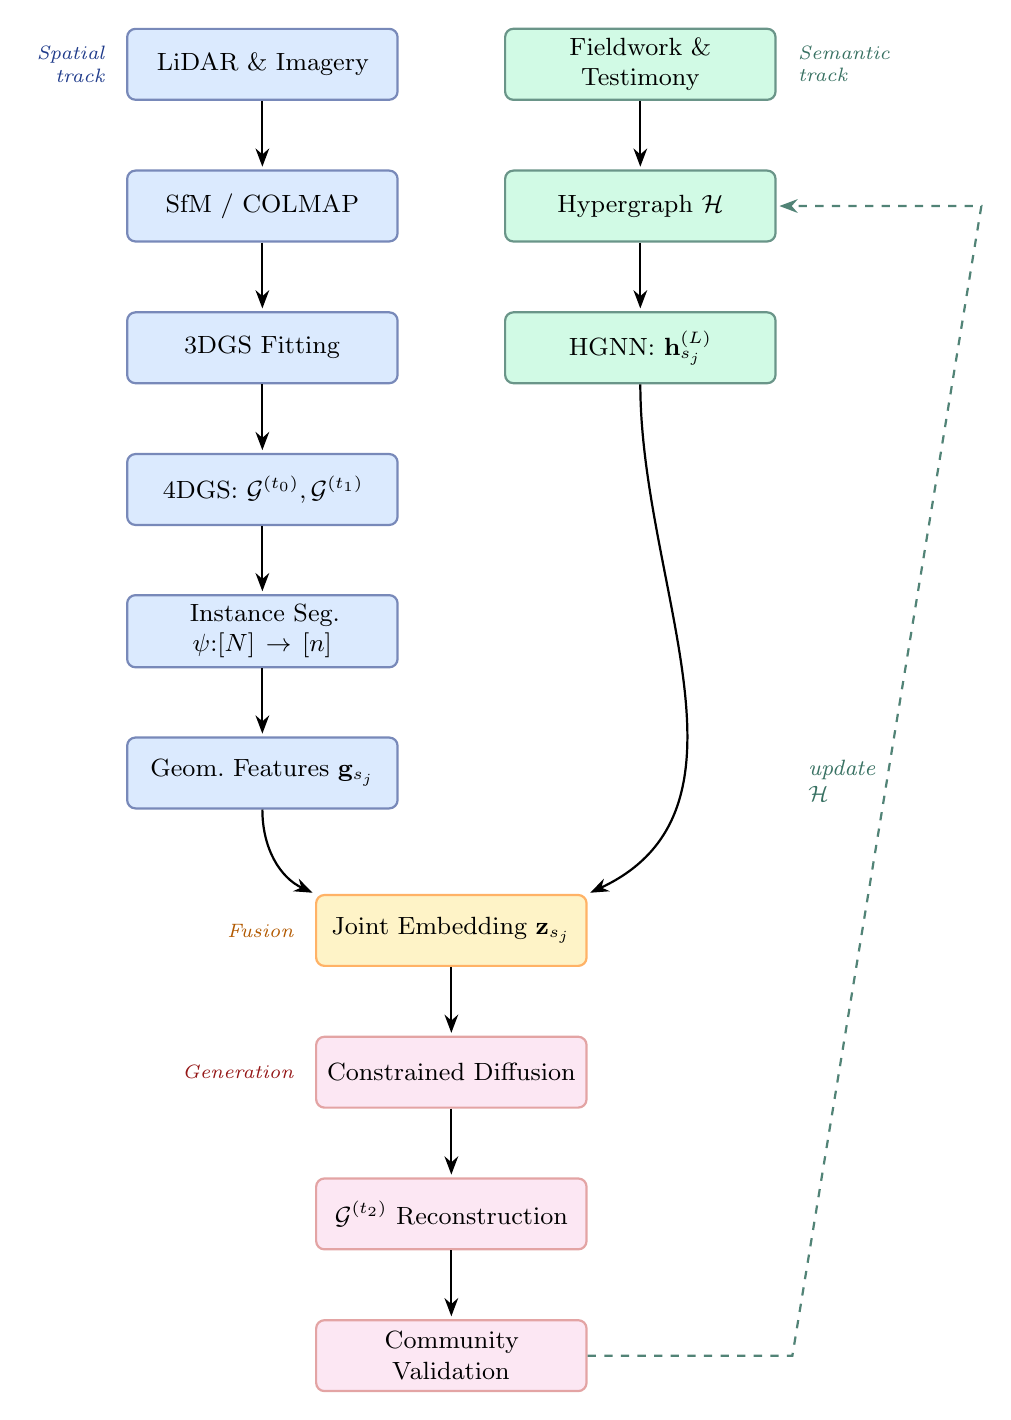
\begin{tikzpicture}[
    >=Stealth,
    box/.style  = {rectangle, rounded corners=3pt,
                   minimum width=3.4cm, minimum height=0.9cm,
                   align=center, font=\small, draw, thick,
                   text width=3.2cm},
    sbox/.style = {box, fill=spatialblue,   draw=darkblue!60},
    hbox/.style = {box, fill=semanticgreen, draw=darkgreen!60},
    fbox/.style = {box, fill=fusionamber,   draw=orange!60},
    gbox/.style = {box, fill=genrose,       draw=eqred!40},
    arr/.style  = {->, thick, shorten >=1pt},
]

%% ── Spatial track: left column, x = -2.4 ────────────────────────────────────
\node[sbox] (lidar) at (-2.4,   0.0)  {LiDAR \& Imagery};
\node[sbox] (sfm)   at (-2.4,  -1.8)  {SfM / COLMAP};
\node[sbox] (gs3d)  at (-2.4,  -3.6)  {3DGS Fitting};
\node[sbox] (gs4d)  at (-2.4,  -5.4)  {4DGS: $\GS^{(t_0)}, \GS^{(t_1)}$};
\node[sbox] (seg)   at (-2.4,  -7.2)  {Instance Seg.\ $\inst{:}[N]\!\to\![n]$};
\node[sbox] (geom)  at (-2.4,  -9.0)  {Geom.\ Features $\gvec_{s_j}$};

%% ── Semantic track: right column, x = +2.4 ──────────────────────────────────
\node[hbox] (field) at ( 2.4,   0.0)  {Fieldwork \& Testimony};
\node[hbox] (hg)    at ( 2.4,  -1.8)  {Hypergraph $\HG$};
\node[hbox] (hgnn)  at ( 2.4,  -3.6)  {HGNN: $\hvec_{s_j}^{(L)}$};

%% ── Fusion: centre ────────────────────────────────────────────────────────────
\node[fbox] (joint) at ( 0.0, -11.0)  {Joint Embedding $\zvec_{s_j}$};

%% ── Generation: centre ───────────────────────────────────────────────────────
\node[gbox] (diff)  at ( 0.0, -12.8)  {Constrained Diffusion};
\node[gbox] (recon) at ( 0.0, -14.6)  {$\GS^{(t_2)}$ Reconstruction};
\node[gbox] (val)   at ( 0.0, -16.4)  {Community Validation};

%% ── Spatial arrows (straight down) ──────────────────────────────────────────
\draw[arr] (lidar) -- (sfm);
\draw[arr] (sfm)   -- (gs3d);
\draw[arr] (gs3d)  -- (gs4d);
\draw[arr] (gs4d)  -- (seg);
\draw[arr] (seg)   -- (geom);

%% ── Spatial to fusion ────────────────────────────────────────────────────────
\draw[arr] (geom.south) to[out=-90, in=155] (joint.north west);

%% ── Semantic arrows (straight down) ─────────────────────────────────────────
\draw[arr] (field) -- (hg);
\draw[arr] (hg)    -- (hgnn);

%% ── Semantic to fusion ───────────────────────────────────────────────────────
\draw[arr] (hgnn.south) to[out=-90, in=25] (joint.north east);

%% ── Generation arrows ────────────────────────────────────────────────────────
\draw[arr] (joint) -- (diff);
\draw[arr] (diff)  -- (recon);
\draw[arr] (recon) -- (val);

%% ── Feedback loop (right side) ───────────────────────────────────────────────
\coordinate (fb1) at ($(val.east)  + (2.6, 0)$);
\coordinate (fb2) at ($(hg.east)   + (2.6, 0)$);
\draw[arr, dashed, darkgreen!70, thick]
    (val.east) -- (fb1) -- (fb2) -- (hg.east);
\node[font=\footnotesize\itshape, darkgreen!80, align=left,
      right=0.08cm of fb1, yshift=7.3cm]
    {update\\$\HG$};

%% ── Track labels ─────────────────────────────────────────────────────────────
\node[font=\scriptsize\itshape, darkblue, align=right,
      left=0.15cm of lidar] {Spatial\\track};
\node[font=\scriptsize\itshape, darkgreen!80, align=left,
      right=0.15cm of field] {Semantic\\track};
\node[font=\scriptsize\itshape, orange!70!black, align=right,
      left=0.15cm of joint] {Fusion};
\node[font=\scriptsize\itshape, eqred!80!black, align=right,
      left=0.15cm of diff]  {Generation};

\end{tikzpicture}
\caption{%
  End-to-end system architecture (vertical layout).
  The \textit{spatial track} (blue, left column) converts LiDAR and
  multi-view imagery into a 4D Gaussian scene and partitions it into
  structural instances with geometric feature vectors $\gvec_{s_j}$.
  The \textit{semantic track} (green, right column) converts community
  fieldwork and oral testimony into the typed governance hypergraph
  $\HG$, whose structural-vertex embeddings $\hvec_{s_j}^{(L)}$ are
  produced by the HGNN.  The two tracks converge at the
  \textit{fusion} stage (amber), which concatenates geometric and
  semantic features into the joint embedding $\zvec_{s_j}$.  The
  \textit{generation} stage (pink) runs constrained diffusion in
  Gaussian parameter space to produce the reconstruction proposal
  $\GS^{(t_2)}$.  Community validation closes the loop: stakeholder
  corrections produce hypergraph update operations (dashed arrow,
  right) that re-enter the semantic track.%
}
\label{fig:architecture}
\end{figure}

% =============================================================================
\section{Preliminaries}
\label{sec:prelim}
% =============================================================================

This section develops all mathematical background required for
\Cref{sec:layer1,sec:layer2,sec:layer3,sec:layer4,sec:layer5}. It is
written for a reader who is technically strong but has not necessarily
encountered formal mathematics as a discipline: we define every object,
operator, and construction the first time it is used. \Cref{sec:prelim_foundations}
introduces the foundational vocabulary (sets, functions, vectors,
matrices, groups, Lagrangians, graphs). \Cref{sec:prelim_3dgs} covers
3D Gaussian splatting. \Cref{sec:prelim_sh} is a self-contained primer
on spherical harmonics. \Cref{sec:prelim_4dgs} covers the 4D extension.
\Cref{sec:prelim_hypergraph} covers hypergraph theory.
\Cref{sec:prelim_hgnn} covers hypergraph neural networks.
\Cref{sec:prelim_gen} covers constrained generative modelling.

\subsection{Mathematical foundations}
\label{sec:prelim_foundations}

This subsection introduces the core mathematical vocabulary used
throughout the paper.

\subsubsection{Sets, functions, and notation}

A \emph{set} $A$ is a collection of distinct objects, called its
\emph{elements}. We write $a \in A$ to mean that $a$ is an element of
$A$, and $a \notin A$ to mean it is not. The \emph{empty set}
$\emptyset$ contains no elements. The set of all subsets of $A$ is
the \emph{power set} $\mathcal{P}(A) = \{B : B \subseteq A\}$; it
has $2^{|A|}$ elements when $A$ is finite.

Standard number sets: $\mathbb{N} = \{0,1,2,\ldots\}$ (natural
numbers), $\mathbb{Z}$ (integers), $\mathbb{Q}$ (rationals),
$\mathbb{R}$ (real numbers), $\mathbb{R}_{>0}$ (positive reals).
The notation $[n] = \{1, 2, \ldots, n\}$ denotes the set of the first
$n$ positive integers.

A \emph{function} $f : A \to B$ assigns to each element $a \in A$
exactly one element $f(a) \in B$. We call $A$ the \emph{domain} and
$B$ the \emph{codomain}. A function is \emph{injective} (one-to-one)
if distinct inputs produce distinct outputs; \emph{surjective}
(onto) if every element of $B$ is hit by some input; and
\emph{bijective} if both. The \emph{composition} of $f : A \to B$ and
$g : B \to C$ is $g \circ f : A \to C$, $(g \circ f)(a) = g(f(a))$.

The notation $\{x \in A : P(x)\}$ means the subset of $A$ consisting
of all $x$ satisfying property $P$. The \emph{intersection}
$A \cap B$ contains elements in both $A$ and $B$; the \emph{union}
$A \cup B$ contains elements in either; the \emph{difference}
$A \setminus B$ contains elements of $A$ not in $B$. The generalised
intersection $\bigcap_{i} A_i$ is the set of elements belonging to
every $A_i$ simultaneously; it plays the role of ``all constraints
simultaneously satisfied'' in \Cref{def:projection}.

\subsubsection{Vectors and the Euclidean space $\mathbb{R}^n$}

A \emph{vector} $\mathbf{x} \in \mathbb{R}^n$ is an ordered list of
$n$ real numbers $\mathbf{x} = (x_1, x_2, \ldots, x_n)^\top$. The
superscript ${}^\top$ (transpose) turns a row into a column; we write
vectors as columns by convention. Addition of vectors and
multiplication by scalars are component-wise:
$\mathbf{x} + \mathbf{y} = (x_1 + y_1, \ldots, x_n + y_n)^\top$
and $\lambda\mathbf{x} = (\lambda x_1, \ldots, \lambda x_n)^\top$.

The \emph{dot product} (inner product) of two vectors is
$\langle \mathbf{x}, \mathbf{y}\rangle = \mathbf{x}^\top \mathbf{y}
= \sum_{i=1}^n x_i y_i \in \mathbb{R}$. The \emph{Euclidean norm}
is $\|\mathbf{x}\| = \sqrt{\mathbf{x}^\top\mathbf{x}}$, the length
of the vector. A \emph{unit vector} satisfies $\|\mathbf{x}\| = 1$.

\subsubsection{Matrices, transposes, and multiplication}

An $m \times n$ matrix $\mathbf{A}$ is a rectangular array of real
numbers with $m$ rows and $n$ columns:
\[
  \mathbf{A} =
  \begin{pmatrix}
    A_{11} & A_{12} & \cdots & A_{1n} \\
    A_{21} & A_{22} & \cdots & A_{2n} \\
    \vdots &        & \ddots & \vdots \\
    A_{m1} & A_{m2} & \cdots & A_{mn}
  \end{pmatrix}.
\]
The \emph{transpose} $\mathbf{A}^\top$ is the $n \times m$ matrix
obtained by swapping rows and columns: $(\mathbf{A}^\top)_{ij} =
A_{ji}$.

\emph{Matrix-vector multiplication}: if $\mathbf{A}$ is $m \times n$
and $\mathbf{x} \in \mathbb{R}^n$, then $\mathbf{A}\mathbf{x} \in
\mathbb{R}^m$ has $i$-th entry $\sum_{j=1}^n A_{ij}x_j$. This
represents a \emph{linear transformation}: $\mathbf{A}$ maps each
input vector $\mathbf{x}$ to an output vector $\mathbf{A}\mathbf{x}$.

\emph{Matrix-matrix multiplication}: if $\mathbf{A}$ is $m \times k$
and $\mathbf{B}$ is $k \times n$, then $\mathbf{C} = \mathbf{A}\mathbf{B}$
is $m \times n$ with entries $C_{ij} = \sum_{\ell=1}^k A_{i\ell}B_{\ell j}$.
This is composition of linear transformations: applying $\mathbf{B}$
first, then $\mathbf{A}$.

A matrix $\mathbf{A}$ is \emph{symmetric} if $\mathbf{A} = \mathbf{A}^\top$.
It is \emph{positive definite} (written $\mathbf{A} \succ 0$) if
$\mathbf{x}^\top \mathbf{A} \mathbf{x} > 0$ for every non-zero
$\mathbf{x}$; geometrically, it defines an ellipsoidal shape in
$\mathbb{R}^n$. The set $\mathcal{S}^n_{++}$ denotes all $n \times n$
real symmetric positive-definite matrices. A symmetric matrix
$\mathbf{A}$ can be decomposed as $\mathbf{A} = \mathbf{U}\boldsymbol{\Lambda}\mathbf{U}^\top$
(eigendecomposition), where $\boldsymbol{\Lambda} = \diag(\lambda_1,\ldots,\lambda_n)$
holds the eigenvalues and $\mathbf{U}$ is orthogonal
($\mathbf{U}\mathbf{U}^\top = \mathbf{I}$).

The \emph{identity matrix} $\mathbf{I}_n$ has ones on the diagonal and
zeros elsewhere; it satisfies $\mathbf{I}\mathbf{x} = \mathbf{x}$ and
$\mathbf{A}\mathbf{I} = \mathbf{I}\mathbf{A} = \mathbf{A}$. The
\emph{trace} of a square matrix is $\tr(\mathbf{A}) = \sum_i A_{ii}$.
The operator $\diag(\mathbf{x})$ constructs the diagonal matrix with
the entries of $\mathbf{x}$ on its diagonal; $\diag(\mathbf{A})$ reads
back the diagonal entries as a vector.

The \emph{half-vectorisation} $\vech(\mathbf{A})$ of a symmetric
$n \times n$ matrix stacks the lower-triangular entries (including
the diagonal) into a vector of length $n(n+1)/2$. It is used in
\Cref{def:geom_feature} to compactly represent the second-moment
matrix of a structural instance.

\subsubsection{Groups and the rotation group $\mathrm{SO}(3)$}

A \emph{group} $(G, \cdot)$ is a set $G$ equipped with an associative
binary operation $\cdot$ that has an identity element $e$ (satisfying
$e \cdot g = g \cdot e = g$ for all $g$) and inverses ($g \cdot g^{-1}
= e$ for every $g$). Groups formalise the notion of symmetry:
rotations, reflections, and translations are all groups.

The \emph{special orthogonal group}
$\SO(3) = \{\mathbf{R} \in \mathbb{R}^{3\times3} : \mathbf{R}\mathbf{R}^\top = \mathbf{I},\;
\det(\mathbf{R}) = 1\}$
is the group of rotations in three dimensions. Every $\mathbf{R} \in
\SO(3)$ is a $3 \times 3$ matrix that rotates vectors without
stretching or reflecting them: $\|\mathbf{R}\mathbf{x}\| = \|\mathbf{x}\|$
for all $\mathbf{x}$. The group operation is matrix multiplication;
the inverse of $\mathbf{R}$ is $\mathbf{R}^\top$.

In practice, elements of $\SO(3)$ are stored as \emph{unit
quaternions} $\mathbf{q} = (q_w, q_x, q_y, q_z)$ with
$\|\mathbf{q}\| = 1$, because quaternions avoid the coordinate
singularity of Euler angles and are more efficient to differentiate
through during gradient-based optimisation.

The \emph{special Euclidean group}
$\SE(3) = \SO(3) \ltimes \mathbb{R}^3$
is the group of rigid-body motions (rotations plus translations).
An element $(\mathbf{R}, \mathbf{t}) \in \SE(3)$ transforms a point
$\mathbf{x} \in \mathbb{R}^3$ as $\mathbf{x} \mapsto \mathbf{R}\mathbf{x} + \mathbf{t}$.
This is the natural group of transformations for camera poses and
scene alignments.

\subsubsection{Optimisation, $\arg\min$, and $\arg\max$}

Given a function $f : \mathcal{X} \to \mathbb{R}$, the \emph{minimum
value} is $\min_{x \in \mathcal{X}} f(x)$ and the \emph{minimiser}
(the point achieving it) is
\[
  \argmin_{x \in \mathcal{X}} f(x)
  = \{x \in \mathcal{X} : f(x) \leq f(y)\;\forall y \in \mathcal{X}\}.
\]
The analogous notation for maximisation is $\argmax$. When the
minimiser is unique, $\argmin$ returns a single point; in general it
is a set. In \Cref{def:recon_problem}, $\argmin$ returns the
reconstruction scene $\GS'$ that minimises the total loss, treating
all Gaussian parameters as decision variables.

The \emph{penalty method} for constrained optimisation replaces a
hard constraint $c(\mathbf{x}) \leq 0$ with an additional term in
the objective: $\min_{\mathbf{x}} f(\mathbf{x}) + \lambda \max(0, c(\mathbf{x}))^2$.
The parameter $\lambda \geq 0$ trades off between minimising $f$ and
satisfying the constraint: when $\lambda$ is large, violations of
$c(\mathbf{x}) \leq 0$ are heavily penalised. As $\lambda \to \infty$,
solutions of the penalised problem converge to solutions of the
original constrained problem.

\subsubsection{The Lagrangian}

The \emph{Lagrangian} of a constrained optimisation problem
\[
  \min_{\mathbf{x}} f(\mathbf{x})
  \quad \text{subject to} \quad c_i(\mathbf{x}) = 0, \; i = 1,\ldots,m
\]
is the function
$\mathcal{L}(\mathbf{x}, \boldsymbol{\mu})
= f(\mathbf{x}) + \sum_{i=1}^m \mu_i c_i(\mathbf{x})$,
where $\boldsymbol{\mu} = (\mu_1, \ldots, \mu_m)$ are called
\emph{Lagrange multipliers}. The Lagrangian converts a constrained
problem into an unconstrained one: at a solution, $\nabla_{\mathbf{x}}
\mathcal{L} = 0$ and $c_i(\mathbf{x}) = 0$, expressing the fact that
the gradient of $f$ must be a linear combination of the gradients of
the constraints. In \Cref{sec:layer4_objective}, we note that the
penalty-weighted total loss $\Ltot$ is the Lagrangian relaxation of
the hard-constrained reconstruction problem \eqref{eq:constrained},
with $\lambda_1$ and $\lambda_2$ playing the role of multipliers.

\subsubsection{Probability and expectation}

A \emph{random variable} $X$ takes values in some set $\mathcal{X}$
with a probability distribution. For continuous $X$ with density
$p(x)$, the \emph{expectation} (mean value) is
$\E[X] = \int x\,p(x)\,\dd x$, and the \emph{variance} measures
spread: $\Var[X] = \E[(X - \E[X])^2]$. For a Gaussian random variable
$X \sim \mathcal{N}(\boldsymbol{\mu}, \boldsymbol{\Sigma})$ in
$\mathbb{R}^n$, $\E[X] = \boldsymbol{\mu}$ and
$\Var[X] = \boldsymbol{\Sigma}$ (the covariance matrix).

A \emph{conditional distribution} $p(X | Y = y)$ describes the
distribution of $X$ given that $Y$ takes the value $y$. Conditional
distributions pervade the generative model of \Cref{sec:layer4_arch},
where the reverse diffusion process is conditioned on the joint
embedding $\mathbf{Z}$.

\subsubsection{Graphs}

A \emph{graph} $G = (V, E)$ consists of a \emph{vertex set} $V$
(a finite set of nodes) and an \emph{edge set}
$E \subseteq \{\{u, v\} : u, v \in V, u \neq v\}$ of unordered pairs
of distinct vertices. An edge $\{u, v\}$ represents a pairwise
relation between $u$ and $v$: in a road network, vertices are
intersections and edges are roads; in a social network, vertices are
people and edges are friendships.

A \emph{directed graph} has edges $E \subseteq V \times V$ that point
from a source to a target. A \emph{weighted graph} assigns a real
number $w_e \in \mathbb{R}$ to each edge. A graph is
\emph{connected} if there is a path between any two vertices.

The \emph{adjacency matrix} $\mathbf{A} \in \{0,1\}^{|V| \times |V|}$
has $A_{uv} = 1$ if $\{u,v\} \in E$ and $A_{uv} = 0$ otherwise.
The \emph{degree} of vertex $v$ is $d(v) = \sum_{u} A_{uv}$, the
number of edges incident to $v$.

Graphs model \emph{binary} relations. The governance relations in our
framework are fundamentally \emph{multi-way}: a single water-sharing
rule links one channel, three terraces, and two households
simultaneously. This motivates the generalisation to hypergraphs,
introduced formally in \Cref{sec:prelim_hypergraph}.

\subsection{Three-dimensional Gaussian splatting}
\label{sec:prelim_3dgs}

We begin with the representation introduced by Kerbl
et al.~\cite{kerbl2023gaussian}, which provides both the geometric
backbone and the rendering mechanism for our framework.

\begin{definition}[3D Gaussian]
\label{def:gaussian}
A \emph{3D Gaussian} is a tuple
\[
  g = \bigl({\boldsymbol\mu},\, {\boldsymbol\Sigma},\, \mathbf{c},\,
            \alpha\bigr),
\]
where ${\boldsymbol\mu} \in \mathbb{R}^3$ is the centre of mass in
world-space coordinates; ${\boldsymbol\Sigma} \in \mathcal{S}^3_{++}$
(the cone of $3\!\times\!3$ real symmetric positive-definite matrices)
is the spatial covariance, encoding the size and orientation of the
Gaussian ellipsoid; $\mathbf{c}: \mathbb{S}^2 \to \mathbb{R}^3$ is a
view-dependent colour function represented by a finite truncation of
the spherical harmonic basis (explained in full in
\Cref{sec:prelim_sh}); and $\alpha \in (0, 1)$ is the opacity.
\end{definition}

\begin{remark}[World-space and the two spheres]
\label{rem:worldspace}
The phrase \emph{world-space} refers to the local Euclidean coordinate
frame $\mathbb{R}^3$ established by the SfM reconstruction of the
scene. Its origin is placed, by convention, at the centroid of the
recovered sparse point cloud (roughly the centre of the reconstructed
village), and its axes are determined by the bundle-adjustment
optimisation, with no fixed orientation relative to geographic north or
local vertical. Positions in this frame are measured in metres and span
a few hundred metres at most.

Two distinct spheres $\mathbb{S}^2$ appear in the framework, and they
must not be confused with each other or with the sphere of the Earth.
\begin{enumerate}[leftmargin=2em]
  \item \textbf{The sphere of viewing directions.} The unit 2-sphere
    $\mathbb{S}^2 = \{\mathbf{x} \in \mathbb{R}^3 : \|\mathbf{x}\| = 1\}$
    appearing in $\mathbf{c} : \mathbb{S}^2 \to \mathbb{R}^3$ is the
    set of all unit vectors in the world-space frame $\mathbb{R}^3$.
    A point on this sphere represents the \emph{direction} from which
    a Gaussian is observed by a camera. It is a 2-dimensional compact
    manifold whose geometry is entirely intrinsic to the local
    reconstruction coordinate frame.
  \item \textbf{Earth's sphere.} The geographic sphere on which the
    High Atlas villages actually reside is a sphere of radius
    $\approx 6{,}371\,\mathrm{km}$, parameterised by latitude and
    longitude. The villages are \emph{points} on this sphere; their
    local tangent plane is the ambient $\mathbb{R}^3$ in which the
    reconstruction lives. The geographic sphere does not appear
    anywhere in the 3DGS or hypergraph mathematics; it enters only
    in the ground-control-point georeferencing of
    \Cref{sec:fieldwork_drone}, where reconstruction coordinates are
    aligned to a geodetic datum (WGS~84).
\end{enumerate}
Both spheres are topologically $\mathbb{S}^2$, but they operate at
completely different spatial scales and serve completely different
mathematical roles.
\end{remark}

\noindent
The covariance ${\boldsymbol\Sigma}$ is stored in factored form
${\boldsymbol\Sigma} = \mathbf{R}\mathbf{S}\mathbf{S}^\top\mathbf{R}^\top$,
where $\mathbf{R} \in \SO(3)$ parameterises orientation as a unit
quaternion and $\mathbf{S} = \diag(s_1, s_2, s_3)$ with $s_i > 0$
parameterises scale. This factorisation ensures positive definiteness
under unconstrained gradient descent.

\begin{definition}[Gaussian scene]
\label{def:scene}
A \emph{Gaussian scene} is a finite multi-set
$\GS = \{g_k\}_{k=1}^N$ of 3D Gaussians. Each element $g_k$ has
its own parameters $({\boldsymbol\mu}_k, {\boldsymbol\Sigma}_k,
\mathbf{c}_k, \alpha_k)$.
\end{definition}

\paragraph{Rendering.}
For a camera with projection matrix $\mathbf{P} \in \mathbb{R}^{3\times4}$
and world-to-camera transform $\mathbf{W} \in \SE(3)$, each Gaussian
$g_k$ is projected to a 2D Gaussian with mean
${\boldsymbol\mu}_k^{2D} = \pi(\mathbf{P}\mathbf{W}{\boldsymbol\mu}_k)$
and covariance
${\boldsymbol\Sigma}_k^{2D} = \mathbf{J}\mathbf{W}{\boldsymbol\Sigma}_k
\mathbf{W}^\top\mathbf{J}^\top$,
where $\mathbf{J}$ is the Jacobian of the projective transformation
at $\mathbf{W}{\boldsymbol\mu}_k$. Pixel colours are computed by
alpha-compositing Gaussians sorted by increasing depth:
\begin{equation}
  \hat{C}(p) = \sum_{k=1}^{N} \mathbf{c}_k(\mathbf{d})
  \,\alpha_k
  \exp\!\Bigl(-\tfrac{1}{2}
    (p - {\boldsymbol\mu}_k^{2D})^\top
    ({\boldsymbol\Sigma}_k^{2D})^{-1}
    (p - {\boldsymbol\mu}_k^{2D})\Bigr)
  \prod_{j < k}\bigl(1 - \alpha_j\bigr),
  \label{eq:rendering}
\end{equation}
where $\mathbf{d}$ is the viewing direction at pixel $p$ and products
over $j < k$ accumulate transmittance over the sorted Gaussians in
front of $k$.

\paragraph{Training objective.}
Given a set of posed input images $\{(I_i, \Pi_i)\}_{i=1}^M$ (image and
camera pose), the scene $\GS$ is optimised by minimising
\begin{equation}
  \mathcal{L}_{\text{photo}} = \sum_{i=1}^{M}
  \Bigl[
    (1 - \lambda_{\mathrm{SSIM}})
    \norm{I_i - \hat{I}_i(\GS)}_1
    + \lambda_{\mathrm{SSIM}}
    \bigl(1 - \mathrm{SSIM}(I_i, \hat{I}_i(\GS))\bigr)
  \Bigr],
  \label{eq:photo_loss}
\end{equation}
where $\hat{I}_i$ is rendered from pose $\Pi_i$ via \eqref{eq:rendering}
and $\lambda_{\mathrm{SSIM}} \approx 0.2$ in practice. Gaussians are
adaptively densified and pruned during optimisation to allocate capacity
where the photometric residual is largest.

\subsection{Spherical harmonics and view-dependent colour}
\label{sec:prelim_sh}

\noindent
This subsection provides a self-contained introduction to spherical
harmonics for readers approaching the topic for the first time. The
material is necessary to understand why the colour function
$\mathbf{c} : \mathbb{S}^2 \to \mathbb{R}^3$ in \Cref{def:gaussian}
takes the form it does, and why the specific sphere $\mathbb{S}^2$
that appears here is the sphere of viewing directions in local
world-space, not any geographic sphere.

\paragraph{Why view-dependent colour?}
A physical surface does not emit or reflect a single colour
uniformly in all directions. The plastered earthen walls of a High
Atlas kasbah appear warm ochre on the sunlit south face, cool grey
in shadow, and have a faint specular sheen at glancing angles where
the mica in the clay catches the light. A bidirectional reflectance
distribution function (BRDF) captures this: it assigns to each
incoming light direction and outgoing viewing direction a reflected
radiance. In the 3DGS setting, the incoming light is not modelled
explicitly; instead, each Gaussian stores a \emph{view-dependent
colour function} $\mathbf{c}(\mathbf{d})$ that directly maps the
viewing direction $\mathbf{d} \in \mathbb{S}^2$ to an RGB colour
response. If a single constant colour were stored per Gaussian, the
rendered image would be flat and viewpoint-independent. The spherical
harmonic parameterisation provides a compact and differentiable family
of functions on $\mathbb{S}^2$ that can represent realistic
view-dependent appearance at low computational cost.

\paragraph{Functions on the unit sphere.}
A \emph{viewing direction} is a unit vector
$\mathbf{d} \in \mathbb{R}^3$ with $\|\mathbf{d}\| = 1$. The set of
all such vectors is the unit 2-sphere
$\mathbb{S}^2 = \{\mathbf{x} \in \mathbb{R}^3 : \|\mathbf{x}\| = 1\}$,
a compact 2-dimensional Riemannian manifold. Every point on
$\mathbb{S}^2$ can be parameterised by spherical coordinates
$(\theta, \varphi)$ with polar angle $\theta \in [0, \pi]$ and
azimuthal angle $\varphi \in [0, 2\pi)$ via the embedding
\[
  \mathbf{d} = (\sin\theta\cos\varphi,\; \sin\theta\sin\varphi,\;
                \cos\theta).
\]
We want to represent an arbitrary square-integrable function
$f : \mathbb{S}^2 \to \mathbb{R}$ as an infinite series. To do this,
we need an orthonormal basis for the Hilbert space
$L^2(\mathbb{S}^2)$ of square-integrable functions on the sphere,
equipped with the inner product
\[
  \langle f, g \rangle
  = \int_{\mathbb{S}^2} f(\mathbf{d})\,g(\mathbf{d})\,\dd\omega,
\]
where $\dd\omega = \sin\theta\,\dd\theta\,\dd\varphi$ is the
standard area element on $\mathbb{S}^2$.

\paragraph{The Laplace--Beltrami operator.}
Just as the Fourier basis on the circle $\mathbb{S}^1$ consists of
the eigenfunctions of the ordinary second-derivative operator
$\frac{\dd^2}{\dd\theta^2}$, the natural basis for $L^2(\mathbb{S}^2)$
consists of the eigenfunctions of the \emph{Laplace--Beltrami operator}
$\Delta_{\mathbb{S}^2}$, the intrinsic Laplacian of the sphere. In
spherical coordinates,
\begin{equation}
  \Delta_{\mathbb{S}^2} f
  = \frac{1}{\sin\theta}
    \frac{\partial}{\partial\theta}
    \!\left(\sin\theta\,\frac{\partial f}{\partial\theta}\right)
  + \frac{1}{\sin^2\!\theta}\,
    \frac{\partial^2 f}{\partial\varphi^2}.
  \label{eq:lbo}
\end{equation}
This operator arises naturally in the Helmholtz equation on
$\mathbb{R}^3$ when one separates variables in spherical coordinates.

\paragraph{Spherical harmonics as eigenfunctions.}
\begin{definition}[Spherical harmonics]
\label{def:sh}
The \emph{real spherical harmonics} $Y_\ell^m : \mathbb{S}^2 \to \mathbb{R}$,
indexed by non-negative integer degree $\ell \geq 0$ and integer order
$m$ with $-\ell \leq m \leq \ell$, are the real-valued eigenfunctions
of $\Delta_{\mathbb{S}^2}$:
\begin{equation}
  \Delta_{\mathbb{S}^2} Y_\ell^m = -\ell(\ell+1)\,Y_\ell^m.
  \label{eq:sh_eigenvalue}
\end{equation}
They form a complete orthonormal system for $L^2(\mathbb{S}^2)$:
\[
  \langle Y_\ell^m, Y_{\ell'}^{m'} \rangle
  = \delta_{\ell\ell'}\,\delta_{mm'}.
\]
\end{definition}

For each degree $\ell$, there are $2\ell + 1$ harmonics (one for
each allowed value of $m$). Up to degree $L$, there are
$(L+1)^2$ harmonics in total. The eigenvalue $-\ell(\ell+1)$ is the
analogue of $-n^2$ in the Fourier case: higher $\ell$ corresponds to
higher angular frequency, i.e.\ more rapid oscillation over the
sphere's surface.

\paragraph{Explicit formulas.}
The real spherical harmonics are constructed from the associated
Legendre polynomials $P_\ell^{|m|}$ as follows. Let
$K_\ell^m = \sqrt{\frac{(2\ell+1)}{4\pi}\frac{(\ell-|m|)!}{(\ell+|m|)!}}$
be a normalisation constant. Then:
\[
  Y_\ell^m(\theta,\varphi) =
  \begin{cases}
    \sqrt{2}\,K_\ell^m \cos(m\varphi)\,P_\ell^m(\cos\theta)
      & \text{if } m > 0, \\
    K_\ell^0 \,P_\ell^0(\cos\theta)
      & \text{if } m = 0, \\
    \sqrt{2}\,K_\ell^{|m|} \sin(|m|\varphi)\,P_\ell^{|m|}(\cos\theta)
      & \text{if } m < 0.
  \end{cases}
\]
The first four degrees are listed explicitly in
\Cref{tab:sh_explicit}. The degree-$0$ harmonic $Y_0^0$ is a
positive constant: a Gaussian whose colour is described by
$Y_0^0$ alone has the same colour from every viewing direction.
The degree-$1$ harmonics are linear functions of the Cartesian
coordinates $(x, y, z)$ evaluated on $\mathbb{S}^2$, and describe
a smooth directional gradient in colour (the difference between the
sun-facing and shadow-facing sides of a wall). Degree-$2$ harmonics
describe quadratic angular variation (such as highlights at oblique
angles), and degree-$3$ harmonics capture cubic oscillation.

\begin{table}[h]
\centering
\small
\caption{Explicit real spherical harmonics up to degree $\ell = 2$.
Here $x = \sin\theta\cos\varphi$, $y = \sin\theta\sin\varphi$,
$z = \cos\theta$ are the Cartesian coordinates of $\mathbf{d}
\in \mathbb{S}^2$, and all expressions are evaluated at
$\mathbf{d}$.}
\label{tab:sh_explicit}
\begin{tabular}{@{}ccc@{}}
\toprule
Degree $\ell$ & Order $m$ & $Y_\ell^m(\mathbf{d})$ \\
\midrule
0 & 0    & $\tfrac{1}{2}\sqrt{\tfrac{1}{\pi}}$ \\[4pt]
1 & $-1$ & $\tfrac{1}{2}\sqrt{\tfrac{3}{\pi}}\,y$ \\[2pt]
1 & $0$  & $\tfrac{1}{2}\sqrt{\tfrac{3}{\pi}}\,z$ \\[2pt]
1 & $+1$ & $\tfrac{1}{2}\sqrt{\tfrac{3}{\pi}}\,x$ \\[4pt]
2 & $-2$ & $\tfrac{1}{2}\sqrt{\tfrac{15}{\pi}}\,xy$ \\[2pt]
2 & $-1$ & $\tfrac{1}{2}\sqrt{\tfrac{15}{\pi}}\,yz$ \\[2pt]
2 & $0$  & $\tfrac{1}{4}\sqrt{\tfrac{5}{\pi}}\,(2z^2 - x^2 - y^2)$ \\[2pt]
2 & $+1$ & $\tfrac{1}{2}\sqrt{\tfrac{15}{\pi}}\,xz$ \\[2pt]
2 & $+2$ & $\tfrac{1}{4}\sqrt{\tfrac{15}{\pi}}\,(x^2 - y^2)$ \\
\bottomrule
\end{tabular}
\end{table}

\paragraph{The SH expansion and truncation.}
Any $f \in L^2(\mathbb{S}^2)$ admits the expansion
\begin{equation}
  f(\mathbf{d})
  = \sum_{\ell=0}^{\infty} \sum_{m=-\ell}^{\ell}
    c_\ell^m\,Y_\ell^m(\mathbf{d}),
  \quad
  c_\ell^m
  = \int_{\mathbb{S}^2} f(\mathbf{d})\,Y_\ell^m(\mathbf{d})\,\dd\omega.
  \label{eq:sh_expansion}
\end{equation}
This is the spherical analogue of a Fourier series. Truncating at
degree $L$ gives the best $L^2$ approximation to $f$ by a linear
combination of at most $(L+1)^2$ basis functions:
\[
  f_L(\mathbf{d})
  = \sum_{\ell=0}^{L} \sum_{m=-\ell}^{\ell}
    c_\ell^m\,Y_\ell^m(\mathbf{d}).
\]
The approximation error $\|f - f_L\|_{L^2}$ decays as $L \to \infty$;
the rate of decay is governed by the smoothness of $f$ on the sphere.

In 3DGS, the colour function of each Gaussian is truncated at $L = 3$,
giving $(3+1)^2 = 16$ basis functions per colour channel. The choice
$L = 3$ reflects an empirical observation about natural materials:
nearly all view-dependent variation in earthen, stone, and plaster
surfaces is captured by low-degree harmonics. A perfectly diffuse
(Lambertian) surface has colour $\mathbf{c}(\mathbf{d}) = c$ constant
in $\mathbf{d}$, which is exactly described by $Y_0^0$ alone ($L = 0$).
A surface with a directional shading gradient (dark on one side, light
on the other) is well approximated by $L = 1$. Mirror-like specular
highlights, which would require very high $L$, are absent in the
High Atlas earthen-construction materials that form the primary subject
of this framework.

\paragraph{Storage and evaluation in 3DGS.}
Each Gaussian $g_k$ stores, for each colour channel
$c \in \{R, G, B\}$, a vector of $(L+1)^2 = 16$ real coefficients
$\{c_{k,\ell,m}^{(c)}\}_{\ell=0,m=-\ell}^{L,\ell}$.
Given a query viewing direction $\mathbf{d}$, the colour is
evaluated as
\begin{equation}
  \mathbf{c}_k(\mathbf{d})
  = \left[
    \sum_{\ell=0}^{L}\sum_{m=-\ell}^{\ell}
      c_{k,\ell,m}^{(c)}\,Y_\ell^m(\mathbf{d})
  \right]_{c \in \{R,G,B\}}.
  \label{eq:sh_eval}
\end{equation}
The direction $\mathbf{d}$ used in this evaluation is the
\emph{viewing direction in world-space}: the unit vector pointing from
the Gaussian's centre ${\boldsymbol\mu}_k$ toward the camera. It is
computed in the local reconstruction coordinate frame and has no
relation to any geographic direction. The SH coefficients
$c_{k,\ell,m}^{(c)}$ are optimised alongside
${\boldsymbol\mu}_k, {\boldsymbol\Sigma}_k, \alpha_k$ during the
photometric training of \Cref{sec:prelim_3dgs}.

\begin{insightbox}
The key intuition for a reader new to spherical harmonics: they are
to functions on the sphere what the Fourier basis $\{1, \sin\theta,
\cos\theta, \sin 2\theta, \ldots\}$ is to functions on the circle.
The degree $\ell$ controls the angular frequency of the basis
function, exactly as $n$ controls the temporal frequency in
$e^{in\theta}$. Storing 16 SH coefficients per Gaussian (and per
colour channel) is analogous to storing the first 16 Fourier
coefficients of a periodic signal: it captures the smooth
low-frequency variation in colour with direction, while ignoring
high-frequency detail that is imperceptible or absent in natural
materials.
\end{insightbox}

\subsection{The four-dimensional extension}
\label{sec:prelim_4dgs}

Static 3DGS cannot represent a scene that changes over time. Wu
et al.~\cite{wu2024_4dgs} and Yang et al.~\cite{yang2024deformable}
extend the model by endowing each Gaussian with a deformation field.

\begin{definition}[4D Gaussian scene]
\label{def:4dgs}
A \emph{4D Gaussian scene} augments each Gaussian $g_k$ with a
deformation $\mathbf{d}_k : \mathcal{T} \to \mathbb{R}^3$ and a
rotation update $\Delta\mathbf{R}_k : \mathcal{T} \to \SO(3)$, where
$\mathcal{T} \subset \mathbb{R}$ is the time domain. The
time-dependent parameters are
\[
  {\boldsymbol\mu}_k(t) = {\boldsymbol\mu}_k + \mathbf{d}_k(t),
  \qquad
  \mathbf{R}_k(t) = \Delta\mathbf{R}_k(t) \cdot \mathbf{R}_k.
\]
\end{definition}

In continuous-video settings $\mathbf{d}_k(t)$ is parameterised by a
neural deformation network $f_\theta(t, k)$. In our framework
$\mathcal{T}$ is discrete: the temporal domain reduces to three
keyframes $\kf = \{t_0, t_1, t_2\}$ representing three distinct
physical states of the scene, so $\mathbf{d}_k(t)$ is a lookup table
with three entries per Gaussian. We discuss the structure of these
keyframes in \Cref{sec:layer1_keyframes}.

\subsection{Hypergraph theory}
\label{sec:prelim_hypergraph}

Ordinary graphs represent pairwise relations. Governance rules over
High Atlas landscapes are fundamentally multi-way: a single Agdal
water-sharing norm constrains an irrigation channel, multiple terraced
plots, and multiple household lineages simultaneously. A hypergraph
is the natural mathematical setting.

\begin{definition}[Hypergraph]
\label{def:hypergraph}
A \emph{hypergraph} is a pair $H = (V, \mathcal{E})$ where $V$ is a
finite vertex set and $\mathcal{E} \subseteq \mathcal{P}(V) \setminus
\{\emptyset\}$ is a family of non-empty subsets of $V$, called
\emph{hyperedges}. An ordinary graph is the special case in which
every hyperedge has cardinality exactly two.
\end{definition}

\begin{definition}[Incidence matrix]
\label{def:incidence}
The \emph{incidence matrix} of $H = (V, \mathcal{E})$ is the matrix
$\mathbf{B} \in \{0,1\}^{|V| \times |\mathcal{E}|}$ defined by
\[
  B_{ve} = \begin{cases} 1 & \text{if } v \in e, \\ 0 & \text{otherwise.} \end{cases}
\]
\end{definition}

\begin{definition}[Degrees]
The \emph{degree} of a vertex $v$ is
$d(v) = \sum_{e \in \mathcal{E}} B_{ve}$,
the number of hyperedges containing $v$.
The \emph{degree} of a hyperedge $e$ is $\delta(e) = |e|$, its
cardinality. We write $\mathbf{D}_V = \diag(d(v))_{v \in V}$ and
$\mathbf{D}_E = \diag(\delta(e))_{e \in \mathcal{E}}$ for the
corresponding diagonal degree matrices.
\end{definition}

\begin{definition}[Hypergraph Laplacian]
\label{def:laplacian}
Let $\mathbf{W} = \diag(w_e)_{e \in \mathcal{E}}$ assign a positive
weight to each hyperedge. The \emph{normalised hypergraph Laplacian}
is
\[
  \boldsymbol{\Delta} = \mathbf{I}
  - \mathbf{D}_V^{-1/2}\,\mathbf{B}\,\mathbf{W}\,
    \mathbf{D}_E^{-1}\,\mathbf{B}^\top\,\mathbf{D}_V^{-1/2}.
\]
This generalises the Cheeger Laplacian of an ordinary graph and
was introduced by Zhou et al.~\cite{zhou2006learning}.
\end{definition}

\begin{definition}[Typed hypergraph]
\label{def:typed_hypergraph}
A \emph{typed hypergraph} is a tuple
$(V, \mathcal{E}, \phi_V, \phi_E)$ where
$\phi_V : V \to \Tv$ and $\phi_E : \mathcal{E} \to \Te$
assign a \emph{type} to each vertex and hyperedge respectively,
for finite type sets $\Tv$ and $\Te$.
\end{definition}

The type functions allow the relational structure to distinguish, for
example, the edge ``actor $a$ owns structure $s$'' from the edge
``rule $r$ restricts structure $s$ during period $[t^-, t^+]$'',
even though both are hyperedges involving $a$ (or $r$) and $s$.
This distinction matters for message passing, as we see in
\Cref{sec:prelim_hgnn}.

\subsection{Hypergraph neural networks}
\label{sec:prelim_hgnn}

A hypergraph neural network (HGNN) propagates information through
the incidence structure of a hypergraph to compute per-vertex
representations that aggregate both local and global context.

\paragraph{Two-stage message passing.}
The standard HGNN layer performs message passing in two stages.
Let $\hvec_v^{(\ell)} \in \mathbb{R}^{d_\ell}$ denote the embedding
of vertex $v$ at layer $\ell$.

\textit{Stage 1 (vertex-to-hyperedge aggregation).}
For each hyperedge $e \in \mathcal{E}$, compute a hyperedge
representation by aggregating over its member vertices:
\[
  \mathbf{z}_e^{(\ell)}
  = \rho_1\!\left(\bigl\{\hvec_v^{(\ell)} : v \in e\bigr\}\right),
\]
where $\rho_1$ is a permutation-invariant aggregation function (sum,
mean, or a learned multiset function).

\textit{Stage 2 (hyperedge-to-vertex aggregation).}
For each vertex $v$, aggregate the representations of all hyperedges
containing $v$:
\[
  \hvec_v^{(\ell+1)}
  = \sigma\!\left(\mathbf{W}^{(\ell)}\,
    \rho_2\!\left(\bigl\{\mathbf{z}_e^{(\ell)} : v \in e\bigr\}\right)
  \right),
\]
where $\mathbf{W}^{(\ell)} \in \mathbb{R}^{d_{\ell+1} \times d_\ell}$
is a learnable weight matrix and $\sigma$ is a non-linearity.

\paragraph{The AllSet formulation.}
Chien et al.~\cite{chien2022allset} show that both aggregations should
be learned multiset functions to avoid information loss. In AllSet,
$\rho_1$ and $\rho_2$ are each parameterised as
\[
  \rho(\{x_i\}) = \text{MLP}\!\left(\frac{1}{|\{x_i\}|}\sum_i
    \text{MLP}(x_i)\right),
\]
which is a universal approximator over multisets. AllSet strictly
subsumes the simpler hypergraph convolution of Feng
et al.~\cite{feng2019hgnn} and the attention variant of Bai
et al.~\cite{bai2021hypergraph}.

\paragraph{Type-sensitive message passing.}
For a typed hypergraph, we use separate weight matrices and
aggregation functions for each hyperedge type $\tau \in \Te$:
\begin{equation}
  \hvec_v^{(\ell+1)}
  = \sigma\!\left(\sum_{\tau \in \Te}
    \mathbf{W}_\tau^{(\ell)}\,
    \rho_{2,\tau}\!\!\left(\bigl\{
      \mathbf{z}_e^{(\ell)} : v \in e,\;
      \phi_E(e) = \tau
    \bigr\}\right)
  \right).
  \label{eq:typed_hgnn}
\end{equation}
This is the relational generalisation of R-GCN~\cite{schlichtkrull2018modeling}
to the hypergraph setting.

\subsection{Constrained generative modelling}
\label{sec:prelim_gen}

We briefly review the denoising diffusion framework~\cite{ho2020ddpm}
and the role of penalty-based constraint enforcement.

\paragraph{Diffusion models.}
A diffusion model defines a forward process that gradually corrupts
a data sample $x^{(0)}$ over $T$ steps:
\[
  q(x^{(1:T)} | x^{(0)})
  = \prod_{t=1}^{T} q(x^{(t)} | x^{(t-1)}),
  \quad
  q(x^{(t)} | x^{(t-1)}) = \mathcal{N}\!\bigl(x^{(t)};
  \sqrt{1-\beta_t}\,x^{(t-1)}, \beta_t \mathbf{I}\bigr),
\]
and a reverse process $p_\theta$ learned to undo the corruption:
\[
  p_\theta(x^{(0:T)})
  = p(x^{(T)})\prod_{t=1}^{T} p_\theta(x^{(t-1)}|x^{(t)}).
\]
The network $\epsilon_\theta(x^{(t)}, t)$ is trained to predict the
noise $\epsilon$ added at step $t$ via
$\mathcal{L}_{\mathrm{DDPM}} = \E\bigl[\norm{\epsilon -
\epsilon_\theta(x^{(t)}, t)}^2\bigr]$.

\paragraph{Conditioned generation.}
To generate samples consistent with a context $\mathbf{Z}$, the reverse
process is conditioned: $p_\theta(x^{(t-1)} | x^{(t)}, \mathbf{Z})$.
The conditioning signal $\mathbf{Z}$ enters via cross-attention in
the denoising network.

\paragraph{Constraint enforcement.}
Two standard mechanisms enforce constraints during generation. Soft
enforcement adds a constraint penalty $\lambda c(x)$ to the training
loss. Hard enforcement applies a projection operator $\Pi_C : x \mapsto
\argmin_{x' \in C} \norm{x' - x}$ after each denoising step, where $C$
is the feasible set. Hard enforcement guarantees constraint satisfaction
at the cost of potentially disrupting the diffusion trajectory; soft
enforcement is differentiable but provides no guarantee. We use both
in \Cref{sec:layer4}.

% =============================================================================
\section{Layer I: The 4D Gaussian Scene}
\label{sec:layer1}
% =============================================================================

This section formalises the spatial layer of our framework: the geometric
representation of the High Atlas landscape as a 4D Gaussian splat scene
over three temporal keyframes.

\subsection{Scene parameterisation}
\label{sec:layer1_scene}

Let $\kf = (t_0, t_1, t_2)$ be an ordered triple of temporal keyframes
with the following interpretations.
\begin{itemize}[leftmargin=2em]
  \item $t_0$: the \emph{pre-earthquake} state, representing the landscape
    as it existed before 8 September 2023. The principal data source for
    this keyframe is archival and community photography.
  \item $t_1$: the \emph{post-earthquake damaged} state, derived from
    systematic drone survey imagery collected on site.
  \item $t_2$: the \emph{proposed reconstruction} state, produced by
    the generative layer (\Cref{sec:layer4}).
\end{itemize}

\begin{definition}[Temporal Gaussian scene]
\label{def:temporal_scene}
For each keyframe $t \in \kf$, the \emph{temporal Gaussian scene}
is
\[
  \GS^{(t)} = \bigl\{g_k^{(t)}\bigr\}_{k=1}^N,
  \quad
  g_k^{(t)} =
  \bigl({\boldsymbol\mu}_k^{(t)},\;
        {\boldsymbol\Sigma}_k^{(t)},\;
        \mathbf{c}_k^{(t)},\;
        \alpha_k^{(t)}\bigr),
\]
where the parameters at keyframe $t$ are related to a canonical
reference by
\[
  {\boldsymbol\mu}_k^{(t)}
  = {\boldsymbol\mu}_k + \mathbf{d}_k(t),
  \qquad
  \mathbf{R}_k^{(t)} = \Delta\mathbf{R}_k(t) \cdot \mathbf{R}_k.
\]
The deformation $\mathbf{d}_k(t) \in \mathbb{R}^3$ and rotation update
$\Delta\mathbf{R}_k(t) \in \SO(3)$ are stored as three-entry lookup
tables indexed by $t \in \kf$.
\end{definition}

\begin{remark}
We deliberately avoid a continuous neural deformation field for the
temporal axis. The keyframes $t_0$ and $t_1$ represent physically
distinct states separated by a seismic event; interpolating between
them is geophysically meaningless. A lookup table is both simpler and
more faithful to the data-generating process.
\end{remark}

\subsection{Multi-view reconstruction}
\label{sec:layer1_reconstruction}

The scenes $\GS^{(t_0)}$ and $\GS^{(t_1)}$ are estimated from
collections of posed photographs via the pipeline: structure-from-motion
(SfM) to recover camera poses, followed by Gaussian fitting to
minimise the photometric loss \eqref{eq:photo_loss}.

\paragraph{Pose recovery.}
Camera poses are recovered from unordered image collections using
COLMAP~\cite{schonberger2016structure}, which solves the incremental SfM
problem: extract and match SIFT features across images, recover a sparse
3D point cloud via bundle adjustment, and estimate intrinsic and
extrinsic parameters for each camera. For archival and community
photographs contributing to $\GS^{(t_0)}$, the images typically have
unknown camera metadata; COLMAP handles this via focal-length
marginalisation and radial distortion estimation~\cite{snavely2006photo}.

\paragraph{Gaussian fitting.}
Given poses $\{\Pi_i^{(t)}\}_{i=1}^{M_t}$ and corresponding images
$\{I_i^{(t)}\}$, the scene $\GS^{(t)}$ is initialised from the COLMAP
sparse point cloud (one Gaussian per sparse point, identity covariance,
uniform opacity) and then optimised by stochastic gradient descent on
\eqref{eq:photo_loss} with adaptive densification.

\paragraph{Keyframe registration.}
To enable deformation-field computation, $\GS^{(t_0)}$ and $\GS^{(t_1)}$
must be expressed in a common world-coordinate frame. Let
$\mathbf{T}^* \in \SE(3)$ be the rigid alignment minimising the
Chamfer distance between the $t_0$ and $t_1$ mean clouds:
\begin{equation}
  \mathbf{T}^* = \argmin_{\mathbf{T} \in \SE(3)}
  \sum_{k=1}^{N}
  \min_{j} \norm{{\boldsymbol\mu}_k^{(t_0)}
  - \mathbf{T}\,{\boldsymbol\mu}_j^{(t_1)}}^2.
  \label{eq:alignment}
\end{equation}
In practice the damaged scene $\GS^{(t_1)}$ will contain
\emph{additional} Gaussians representing rubble and collapse debris and
\emph{fewer} Gaussians in collapsed structural regions; the Chamfer
objective is robust to this asymmetry. After alignment, all scenes
share a common coordinate system and the deformations
$\mathbf{d}_k(t_1) = {\boldsymbol\mu}_k^{(t_1)} - {\boldsymbol\mu}_k^{(t_0)}$
can be interpreted as displacement vectors encoding earthquake damage.

\subsection{Temporal keyframe structure}
\label{sec:layer1_keyframes}

\begin{definition}[Displacement field]
The \emph{damage displacement field} is the map
\[
  \mathbf{D} : \GS^{(t_0)} \to \mathbb{R}^3,
  \quad
  \mathbf{D}(g_k) = {\boldsymbol\mu}_k^{(t_1)} - {\boldsymbol\mu}_k^{(t_0)},
\]
defined after solving \eqref{eq:alignment}. For Gaussians in structurally
intact regions, $\mathbf{D}(g_k) \approx \mathbf{0}$. Persistent
large-magnitude displacements indicate collapse or debris accumulation.
\end{definition}

\begin{remark}
The keyframe $t_2$ is not given but generated: it is the output of the
constrained generation stage in \Cref{sec:layer4}. Its deformation
$\mathbf{d}_k(t_2)$ represents the proposed reconstruction displacement
from the reference configuration, subject to physical and governance
constraints.
\end{remark}

\subsection{Gaussian instance segmentation}
\label{sec:layer1_seg}

A raw Gaussian scene $\GS$ is an unstructured collection of primitives.
To reason about governance at the level of architectural elements, we
must partition $\GS$ into semantically coherent structural instances.

\begin{definition}[Structural instance]
\label{def:structural_instance}
A \emph{structural instance} $s_j$ is a maximal set of Gaussians that
correspond to a single semantically coherent physical element: a
building, a terrace, a water channel, a threshold, a granary, or a
sacred enclosure. The set $\Struc = \{s_1, \ldots, s_n\}$ partitions
the physical elements of the scene.
\end{definition}

\begin{definition}[Instance assignment map]
\label{def:psi}
The \emph{instance assignment map} is a surjection
$\inst : [N] \to [n]$ such that $\inst(k) = j$ if and only if Gaussian
$g_k$ is assigned to instance $s_j$. The assignment induces a partition
$\{G_{s_j}\}_{j=1}^n$ of $[N]$ by
\[
  \GS_{s_j} = \bigl\{g_k \in \GS : \inst(k) = j\bigr\}.
\]
\end{definition}

The instance map $\inst$ is computed in two stages. First, a
foundation segmentation model~\cite{kirillov2023sam} produces
per-Gaussian semantic label probabilities by projecting each Gaussian
mean into multiple rendered views and aggregating the resulting masks.
Second, Gaussians with the same dominant semantic label that are
spatially adjacent (within a threshold $\epsilon$ in world space) are
merged into a single instance. In highly damaged scenes, this process
requires manual verification of a small subset of instances; we discuss
the annotation interface for this in \Cref{sec:layer5}.

Recent work on Gaussian Grouping~\cite{ye2024gaussian} provides a
differentiable variant in which the instance labels are trained jointly
with the Gaussian parameters, yielding sharper boundaries between
instances. We treat this as an available implementation option; the
formal definition of $\inst$ is independent of the specific algorithm
used to compute it.

\subsection{Structural instance geometry}
\label{sec:layer1_geom}

For each structural instance $s_j$, we compute a compact geometric
feature vector that summarises the spatial and photometric properties
of its constituent Gaussians.

\begin{definition}[Geometric feature]
\label{def:geom_feature}
The \emph{geometric feature} of instance $s_j$ is the vector
$\gvec_{s_j} \in \mathbb{R}^{d_g}$ defined by
\begin{align*}
  \bar{{\boldsymbol\mu}}_{s_j}
  &= \frac{\sum_{k : \inst(k)=j} \alpha_k\,{\boldsymbol\mu}_k}
          {\sum_{k : \inst(k)=j} \alpha_k}
  & \text{(opacity-weighted centroid)},\\
  \mathbf{M}_{s_j}
  &= \frac{\sum_{k : \inst(k)=j} \alpha_k
    ({\boldsymbol\mu}_k - \bar{{\boldsymbol\mu}}_{s_j})
    ({\boldsymbol\mu}_k - \bar{{\boldsymbol\mu}}_{s_j})^\top}
    {\sum_{k : \inst(k)=j} \alpha_k}
  & \text{(second-moment matrix)},\\
  v_{s_j}
  &= \sum_{k : \inst(k)=j} \alpha_k
  & \text{(total opacity)},\\
  \bar{\mathbf{c}}_{s_j}
  &= \frac{1}{|\GS_{s_j}|}\sum_{k : \inst(k)=j} \mathbf{c}_k
  & \text{(mean colour coefficients)}.
\end{align*}
The feature vector is then
$\gvec_{s_j} = \bigl[\bar{{\boldsymbol\mu}}_{s_j}^\top;\;
\vech(\mathbf{M}_{s_j});\; v_{s_j};\; \bar{\mathbf{c}}_{s_j}^\top\bigr]^\top$,
where $\vech$ denotes the half-vectorisation of the symmetric matrix.
\end{definition}

\begin{remark}
The opacity weighting in the centroid and second-moment computations
ensures that lightly contributing Gaussians (those on the periphery of
an instance, often with small $\alpha_k$) do not unduly influence the
geometric summary. The second-moment matrix $\mathbf{M}_{s_j}$ encodes
the extent and orientation of the instance as an ellipsoid, and its
eigenvalue decomposition provides a natural coordinate frame for the
structural element.
\end{remark}

% =============================================================================
\section{Layer II: The Governance Hypergraph}
\label{sec:layer2}
% =============================================================================

The governance hypergraph $\HG = (V, \mathcal{E}, \phi_V, \phi_E)$
is the formal representation of the social, cultural, and normative
context of the landscape. It encodes who governs what, under what rules,
for what reasons, and with what history. This section defines the vertex
and hyperedge taxonomies, derives the incidence structure, treats
temporal governance, and establishes the necessity of conflict-preserving
representation.

\subsection{Vertex taxonomy}
\label{sec:layer2_vertices}

The vertex set $V$ is partitioned into five typed subsets:
\[
  V = \Struc \cup \Act \cup \Nar \cup \Rul \cup \Evt,
\]
with vertex type function $\phi_V : V \to \Tv$,
$\Tv = \{\mathrm{Str}, \mathrm{Act}, \mathrm{Nar}, \mathrm{Rul},
\mathrm{Evt}\}$.

\begin{definition}[Structural vertex]
Each element $s_j \in \Struc$ corresponds directly to a structural
instance in $\Struc$ from \Cref{def:structural_instance}: a building,
terrace, water channel, granary, threshold, or sacred enclosure.
Structural vertices are the primary locus of governance: all other
vertex types interact with the landscape through edges anchored at one
or more structural vertices.
\end{definition}

\begin{definition}[Actor vertex]
Each element $a \in \Act$ represents a governance-relevant agent: an
individual person, a named family lineage
(\textit{tawmat} [\textarabic{تاومات}]), a
household cluster, or a collective institution such as a village council
(\textit{jma\^{a}a} [\textarabic{جماعة}]) or a water-sharing guild. Actor vertices carry
attributes including agent type, approximate lineage depth (number of
generations of documented use), and current residency status.
\end{definition}

\begin{definition}[Narrative vertex]
Each element $n \in \Nar$ is a record unit: a transcribed oral
testimony with speaker provenance, date of recording, and language
(Tachelhit, Tamazight, Darija, or French); or an archival document
(cadastral record, heritage inventory, NGO survey, photographic archive
entry) with source and date. Narrative vertices do not themselves
prescribe governance; they provide evidential grounding for the edges
that do.
\end{definition}

\begin{definition}[Rule vertex]
\label{def:rule_vertex}
Each element $r \in \Rul$ encodes a normative proposition in a
structured form:
\[
  r = (\tau_r,\; C_r,\; [t_r^-, t_r^+],\; \sigma_r,\; \mathcal{P}_r),
\]
where $\tau_r \in \{\mathrm{permission}, \mathrm{prohibition},
\mathrm{obligation}\}$ is the deontic modality; $C_r$ is a
precondition formula (a Boolean expression over vertex attributes and
edge membership); $[t_r^-, t_r^+]$ is the temporal validity interval
(possibly $(-\infty, +\infty)$ for permanent rules); $\sigma_r \in
[0,1]$ is a cultural sensitivity score assigned during community
sessions; and $\mathcal{P}_r \subseteq \Act$ is the set of actors with
the authority to modify or revoke $r$.
\end{definition}

\begin{example}
The Agdal restriction on grazing in the upper Alpine meadows of the
Oukaïmeden is represented as a rule vertex $r_{\mathrm{agdal}}$ with
deontic modality \textit{prohibition}, precondition $C_r :=$
\emph{``the current date falls in the closed-Agdal period''},
temporal validity interval $[1\,\text{April}, 15\,\text{July}]$
(approximate for the High Atlas agdal), sensitivity $\sigma_r = 0.93$
(high), and authority $\mathcal{P}_r$ the village council of the
relevant fraction.
\end{example}

\begin{definition}[Event vertex]
Each element $e_v \in \Evt$ records a historical episode that changed
the semantic status of one or more structural vertices: the original
construction of a building, a fire, an inheritance transfer, the
September 2023 earthquake, or a prior reconstruction. Event vertices
carry a timestamp and a description; they serve as anchors for
temporal reasoning about provenance and prior state.
\end{definition}

\subsection{Hyperedge taxonomy}
\label{sec:layer2_edges}

We define six hyperedge types, collected in $\Te$. The key property
distinguishing each type is the cardinality and type-composition of the
incident vertices.

\begin{definition}[Ownership hyperedge]
$e_{\mathrm{owns}} \subseteq \mathcal{P}(\Act \cup \Struc)$,
with $e_{\mathrm{owns}} \cap \Act \neq \emptyset$ and
$e_{\mathrm{owns}} \cap \Struc \neq \emptyset$.
A single ownership hyperedge encodes a governance claim: the actors in
$e_{\mathrm{owns}} \cap \Act$ assert collective ownership or stewardship
over the structures in $e_{\mathrm{owns}} \cap \Struc$. Collective
claims naturally require hyperedges of cardinality greater than two.
\end{definition}

\begin{definition}[Governance hyperedge]
$e_{\mathrm{gov}} \subseteq \mathcal{P}(\Rul \cup \Struc \cup \Act)$,
with $e_{\mathrm{gov}} \cap \Rul \neq \emptyset$.
A governance hyperedge binds a rule $r \in \Rul$ to the spatial
structures and actors it governs. This is the primary mechanism by
which Agdal norms, water-turn schedules, and land-use restrictions are
attached to spatial elements.
\end{definition}

\begin{definition}[Testimony hyperedge]
$e_{\mathrm{test}} \subseteq \mathcal{P}(\Nar \cup \Struc \cup \Evt)$,
with $e_{\mathrm{test}} \cap \Nar \neq \emptyset$.
A testimony hyperedge links a narrative record $n \in \Nar$ to the
structural elements and historical events it describes, providing an
evidential chain from oral or archival knowledge to the geometric layer.
\end{definition}

\begin{definition}[Co-functional hyperedge]
$e_{\mathrm{cofunc}} \subseteq \mathcal{P}(\Struc)$,
$|e_{\mathrm{cofunc}}| \geq 2$.
A co-functional hyperedge groups structural elements that constitute a
single functional unit: a water channel together with all terraces it
irrigates, or a granary together with the threshing floor and storage
alcoves that compose it. Constraint violations by one member of a
co-functional hyperedge propagate to all members.
\end{definition}

\begin{definition}[Contested hyperedge]
$e_{\mathrm{cont}} \subseteq \mathcal{P}(\Act \cup \Struc)$,
satisfying the additional condition that there exist
$e_{\mathrm{cont}}', e_{\mathrm{cont}}'' \in \mathcal{E}$ with
$\phi_E(e') = \phi_E(e'') = \mathrm{owns}$,
$e' \cap \Struc = e'' \cap \Struc = \{s\}$ for some $s \in \Struc$,
and $e' \cap \Act \neq e'' \cap \Act$.
In plain terms: two or more distinct ownership hyperedges claim the
same structure. We represent the \emph{dispute itself} as an explicit
contested hyperedge $e_{\mathrm{cont}}$ involving all disputing actors
and the contested structure, with a \texttt{status} attribute
$\in \{\mathrm{active}, \mathrm{mediation}, \mathrm{resolved}\}$.
\end{definition}

\begin{definition}[Temporal hyperedge]
$e_{\mathrm{temp}} \subseteq \mathcal{P}(\Evt \cup \Struc)$,
augmented with a timestamp $\tau(e_{\mathrm{temp}}) \in \mathbb{R}$.
A temporal hyperedge records that an event $v_e \in \Evt$ changed
the state of a set of structural elements at time $\tau$. The
sequence of temporal hyperedges incident to a structure $s_j$ forms
its \emph{provenance chain}.
\end{definition}

\begin{figure}[t]
\centering
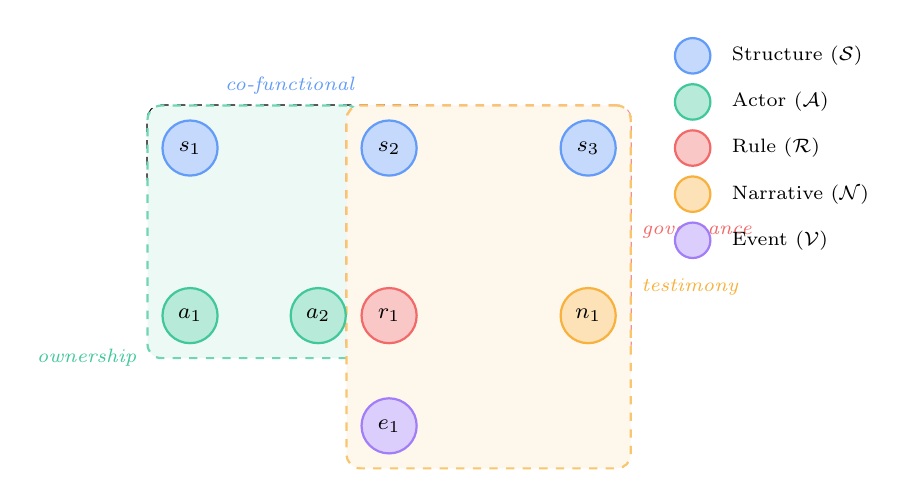
\begin{tikzpicture}[
    >=Stealth,
    vnode/.style = {circle, draw, thick, minimum size=0.7cm,
                    font=\footnotesize, inner sep=1pt},
    str/.style   = {vnode, fill=nodestr!30,  draw=nodestr!80},
    act/.style   = {vnode, fill=nodeact!30,  draw=nodeact!80},
    nar/.style   = {vnode, fill=nodenar!30,  draw=nodenar!80},
    rul/.style   = {vnode, fill=noderul!30,  draw=noderul!80},
    evt/.style   = {vnode, fill=nodeevt!30,  draw=nodeevt!80},
    hedge/.style = {rounded corners=5pt, draw, dashed, thick,
                    inner sep=5pt},
    node distance=1.1cm and 1.3cm,
]

%% ── Nodes ────────────────────────────────────────────────────────────────────
\node[str] (s1) {$s_1$};
\node[str, right=1.8cm of s1] (s2) {$s_2$};
\node[str, right=1.8cm of s2] (s3) {$s_3$};

\node[act, below=1.4cm of s1] (a1) {$a_1$};
\node[act, right=0.9cm of a1] (a2) {$a_2$};

\node[rul, below=1.4cm of s2] (r1) {$r_1$};

\node[nar, below=1.4cm of s3] (n1) {$n_1$};

\node[evt, below=2.8cm of s2] (ev1) {$e_1$};

%% ── Co-functional hyperedge ──────────────────────────────────────────────────
\begin{scope}[on background layer]
  \node[hedge, fill=nodestr!8, fit=(s1)(s2),
        label={[font=\scriptsize\itshape, nodestr!80]above:co-functional}]
        (cf) {};
\end{scope}

%% ── Ownership hyperedge ──────────────────────────────────────────────────────
\begin{scope}[on background layer]
  \node[hedge, fill=nodeact!8, draw=nodeact!60,
        fit=(a1)(a2)(s1),
        label={[font=\scriptsize\itshape,nodeact!80]below left:ownership}]
        (ow) {};
\end{scope}

%% ── Governance hyperedge ─────────────────────────────────────────────────────
\begin{scope}[on background layer]
  \node[hedge, fill=noderul!8, draw=noderul!60,
        fit=(r1)(s2)(s3),
        label={[font=\scriptsize\itshape,noderul!80]right:governance}]
        (gv) {};
\end{scope}

%% ── Testimony hyperedge ──────────────────────────────────────────────────────
\begin{scope}[on background layer]
  \node[hedge, fill=nodenar!8, draw=nodenar!60,
        fit=(n1)(s3)(ev1),
        label={[font=\scriptsize\itshape,nodenar!80]right:testimony}]
        (tv) {};
\end{scope}

%% ── Legend ───────────────────────────────────────────────────────────────────
\matrix[right=0.6cm of s3, ampersand replacement=\&,
        row sep=3pt, column sep=4pt] {
  \node[str, minimum size=0.45cm] {}; \& \node[font=\scriptsize] {Structure ($\Struc$)}; \\
  \node[act, minimum size=0.45cm] {}; \& \node[font=\scriptsize] {Actor ($\Act$)}; \\
  \node[rul, minimum size=0.45cm] {}; \& \node[font=\scriptsize] {Rule ($\Rul$)}; \\
  \node[nar, minimum size=0.45cm] {}; \& \node[font=\scriptsize] {Narrative ($\Nar$)}; \\
  \node[evt, minimum size=0.45cm] {}; \& \node[font=\scriptsize] {Event ($\Evt$)}; \\
};

\end{tikzpicture}
\caption{%
  A fragment of the governance hypergraph $\HG$. Structural vertices
  $s_1, s_2, s_3$ (blue) are linked by a co-functional hyperedge
  (the dashed box enclosing $s_1, s_2$). An ownership hyperedge binds
  actors $a_1, a_2$ and structure $s_1$. A governance hyperedge binds
  rule $r_1$ to structures $s_2, s_3$. A testimony hyperedge binds
  narrative $n_1$ to structure $s_3$ and event $e_1$. Node colour
  encodes vertex type; the same structure node participates in
  multiple hyperedges simultaneously.%
}
\label{fig:hypergraph_taxonomy}
\end{figure}

\subsection{The incidence structure}
\label{sec:layer2_incidence}

Given the typed hypergraph $\HG$, the incidence matrix $\mathbf{B}$
(\Cref{def:incidence}) can be decomposed by edge type. For each
$\tau \in \Te$, define the \emph{type-restricted incidence matrix}
\[
  \mathbf{B}^\tau_{ve}
  = B_{ve} \cdot \mathbf{1}[\phi_E(e) = \tau],
\]
so that $\mathbf{B} = \sum_{\tau \in \Te} \mathbf{B}^\tau$.
This decomposition underlies the type-sensitive HGNN
of \eqref{eq:typed_hgnn}.

The \emph{governance-restricted} incidence $\mathbf{B}^{\mathrm{gov}}$
deserves special attention: its rows indexed by structural vertices
$s_j \in \Struc$ encode which governance rules directly constrain
each structure. For a structural vertex $s_j$,
\[
  \bigl[\mathbf{B}^{\mathrm{gov}}\bigr]_{s_j,:}
  = \mathbf{1}\bigl[\exists r \in \Rul :
    (r \in e) \wedge (s_j \in e) \wedge
    (\phi_E(e) = \mathrm{gov})\bigr].
\]
This row vector is the primary input to the governance constraint loss
in \Cref{sec:layer4_gov_loss}.

\subsection{Temporal governance}
\label{sec:layer2_temporal}

Amazigh governance norms are not time-homogeneous. The Agdal system
imposes seasonal restrictions; inheritance transfers modify ownership
at discrete points in time; damage events alter the physical and
normative status of structures.

\begin{definition}[Temporally active rule]
\label{def:active_rule}
At real calendar time $\tau$, a rule vertex $r \in \Rul$ is
\emph{active} if and only if
\[
  \tau \in [t_r^-, t_r^+]
  \quad \text{and} \quad
  C_r \text{ evaluates to } \mathrm{True}
  \text{ given the current state of } \HG.
\]
The set of active rules at time $\tau$ is
$\Rul_\tau = \{r \in \Rul : r \text{ is active at } \tau\}$.
\end{definition}

\begin{definition}[Temporally active governance hyperedge]
A governance hyperedge $e \in \mathcal{E}$ with $\phi_E(e) =
\mathrm{gov}$ is \emph{active} at time $\tau$ if the rule vertex
$r = e \cap \Rul$ (there is exactly one rule per governance
hyperedge) belongs to $\Rul_\tau$.
\end{definition}

\begin{remark}
The constraint layer in \Cref{sec:layer4} evaluates governance
compliance at the nominal reconstruction time $\tau_{\mathrm{rec}}$,
which is set to the expected construction completion date. Rules
whose validity intervals do not contain $\tau_{\mathrm{rec}}$ are
excluded from the constraint loss. Seasonal restrictions that
overlap with the reconstruction period therefore impose actual
constraints on the generated design.
\end{remark}

\subsection{Conflict-preserving representation}
\label{sec:layer2_conflict}

A central design principle of our framework is that contested ownership
claims must be represented explicitly and preserved intact rather than
collapsed into a single ``resolved'' state. We now make this principle
precise and prove it necessary.

\begin{definition}[Conflict pair]
\label{def:conflict_pair}
A \emph{conflict pair} over structure $s_j \in \Struc$ is a pair of
distinct ownership hyperedges $(e', e'') \in \mathcal{E}^2$ such that
\begin{enumerate}[leftmargin=2.5em, label=(\roman*)]
  \item $\phi_E(e') = \phi_E(e'') = \mathrm{owns}$,
  \item $s_j \in e' \cap e''$,
  \item $e' \cap \Act \neq e'' \cap \Act$ (distinct claimant sets).
\end{enumerate}
\end{definition}

\begin{definition}[Collapsed hypergraph]
\label{def:collapsed}
Given a hypergraph $\HG$ containing a conflict pair $(e', e'')$
over $s_j$, the \emph{collapsed} hypergraph $\overline{\HG}$ is
obtained by removing $e'$ and $e''$ and inserting a single ownership
hyperedge $\bar{e}$ with $\bar{e} \cap \Act = e' \cap \Act$ (i.e.,
resolving in favour of one claimant). Collapsing in favour of $e''$
is defined analogously.
\end{definition}

\begin{proposition}[Necessity of conflict preservation]
\label{prop:conflict_necessity}
Let $C_{\HG}$ denote the set of governance-feasible reconstruction
scenes for hypergraph $\HG$, defined as
\[
  C_{\HG} = \bigl\{\GS' : \Lgov(\GS', \HG) = 0\bigr\},
\]
where $\Lgov$ is the governance constraint loss from \Cref{sec:layer4}.
For any conflict pair $(e', e'')$ in $\HG$, let $\overline{\HG}$ be
the collapsed hypergraph favouring $e'$. Then in general
$C_{\HG} \subset C_{\overline{\HG}}$, i.e., collapsing expands the
feasible set, admitting designs that violate the original contested claim.
\end{proposition}

\begin{proof}
Under the collapsed hypergraph $\overline{\HG}$, actor set
$e'' \cap \Act$ holds no ownership claim over $s_j$. Therefore any
design that, under $\HG$, would violate $e''$'s claim (e.g., by
constructing a wall that blocks access the $e''$-claimant lineage
historically enjoyed) is no longer recognised as a constraint violation
in $C_{\overline{\HG}}$. Formally, let $\GS^*$ be any scene satisfying
$\Lgov(\GS^*, \HG) = 0$. By the constraint structure, $\GS^*$ must
simultaneously respect both $e'$ and $e''$, so it belongs to
$C_{\HG}$. But there exist scenes $\GS^{**}$ with
$\Lgov(\GS^{**}, \overline{\HG}) = 0$ that violate $e''$'s claim,
hence $\GS^{**} \notin C_{\HG}$. Thus $C_{\HG} \subsetneq
C_{\overline{\HG}}$.
\end{proof}

\begin{insightbox}
\Cref{prop:conflict_necessity} formalises a key social fact: by
collapsing a contested claim, the design system implicitly decides the
dispute on behalf of the community. This is governance by technical
default. Conflict-preserving representation ensures that the set of
admissible reconstructions is the intersection of all plausible
governance interpretations, not the union of one.
\end{insightbox}

\subsection{Formal properties of the governance hypergraph}
\label{sec:layer2_properties}

We close this section with two structural properties that relate to
the soundness and completeness of the governance encoding.

\begin{definition}[Governance consistency]
The hypergraph $\HG$ is \emph{governance-consistent} if no rule vertex
$r \in \Rul$ is simultaneously active and its logical negation is
implied by the current hyperedge structure. Informally, no pair of
active governance edges simultaneously requires and prohibits the same
spatial configuration.
\end{definition}

\begin{definition}[Structural coverage]
The hypergraph $\HG$ is \emph{structurally complete} with respect to
an instance set $\Struc$ if every structural vertex $s_j \in \Struc$
is incident to at least one ownership hyperedge and at least one
testimony hyperedge. Structural completeness is the minimum standard
required before committing to constrained generation.
\end{definition}

\begin{remark}
In practice $\HG$ will not be structurally complete after the first
round of community annotation. The active learning criterion in
\Cref{sec:layer5} prioritises annotation of structurally incomplete
vertices.
\end{remark}

% =============================================================================
\section{Layer III: Gaussian-to-Hypergraph Alignment}
\label{sec:layer3}
% =============================================================================

The spatial layer $\GS$ and the semantic layer $\HG$ are coupled through
two operations: the instance assignment map $\inst$ (\Cref{def:psi}),
which routes each Gaussian to a structural vertex, and the joint
embedding, which fuses geometric and semantic information at each
structural instance.

\subsection{The instance alignment}
\label{sec:layer3_alignment}

The structural instance vertices $\Struc \subset V$ are in bijective
correspondence with the structural instances $\{s_1, \ldots, s_n\}$
of the spatial layer: each $s_j \in \Struc$ identifies both a
hypergraph vertex and a set of Gaussians $\GS_{s_j}$.
The instance assignment map $\inst : [N] \to [n]$
(\Cref{def:psi}) therefore induces a map
$\tilde{\inst} : \GS \to \Struc$ defined by
$\tilde{\inst}(g_k) = s_{\inst(k)}$.

This coupling has two consequences. First, any attribute of a
structural vertex $s_j$ in the hypergraph (ownership claims, active
rules, testimony records) is semantically associated with the set of
Gaussians $\GS_{s_j}$. Second, any physical modification of the
Gaussians in $\GS_{s_j}$ (in the generative stage) is subject to the
governance constraints incident at $s_j$.

\subsection{Geometric aggregation}
\label{sec:layer3_geom_agg}

Each structural vertex $s_j$ receives a geometric feature vector
$\gvec_{s_j}$ from \Cref{def:geom_feature}. For the post-earthquake
keyframe $t_1$, this feature vector is extended with a damage indicator:
\[
  \gvec_{s_j}^{(t_1)}
  = \bigl[\gvec_{s_j};\;
    d_{s_j};\;
    \bar{\mathbf{D}}_{s_j}\bigr]^\top,
\]
where $d_{s_j} = \frac{1}{|\GS_{s_j}|}
\sum_{k:\inst(k)=j}\norm{\mathbf{D}(g_k)}$ is the mean damage
displacement magnitude for the instance, and
$\bar{\mathbf{D}}_{s_j} = \frac{1}{|\GS_{s_j}|}
\sum_{k:\inst(k)=j}\mathbf{D}(g_k)$
is the mean damage displacement vector. Large $d_{s_j}$ indicates
collapse or severe displacement; near-zero $d_{s_j}$ indicates
structural survival.

\subsection{Joint embedding}
\label{sec:layer3_joint}

\begin{definition}[Joint embedding]
\label{def:joint_embed}
Let $\hvec_{s_j}^{(L)} \in \mathbb{R}^{d_h}$ be the HGNN output
embedding of structural vertex $s_j$ after $L$ message-passing layers,
computed via \eqref{eq:typed_hgnn}. Let
$\gvec_{s_j} \in \mathbb{R}^{d_g}$ be the geometric feature of
\Cref{def:geom_feature}. The \emph{joint embedding} of instance $s_j$
is
\begin{equation}
  \zvec_{s_j}
  = \text{MLP}_\phi\!\bigl(
      \mathbf{W}_h\,\hvec_{s_j}^{(L)} \,\|\, \mathbf{W}_g\,\gvec_{s_j}
    \bigr)
    \in \mathbb{R}^{d_z},
  \label{eq:joint_embed}
\end{equation}
where $\mathbf{W}_h \in \mathbb{R}^{d_z/2 \times d_h}$ and
$\mathbf{W}_g \in \mathbb{R}^{d_z/2 \times d_g}$ are linear
projections, $\|$ denotes concatenation, and $\text{MLP}_\phi$
is a two-layer network with parameters $\phi$. The matrix
$\mathbf{Z} \in \mathbb{R}^{n \times d_z}$ stacks all joint
embeddings row-wise.
\end{definition}

\begin{remark}
The projection dimensions $d_z/2$ for each modality enforce a balanced
fusion prior before the MLP. An alternative is to use a cross-attention
mechanism over the Gaussian point cloud conditioned on the HGNN
embeddings; we adopt the simpler concatenation scheme here and note
the attention variant as an open architectural question
(\Cref{sec:open}).
\end{remark}

The joint embedding $\zvec_{s_j}$ now carries, for each structural
instance: (i) its geometric shape, extent, opacity, and photometric
character; (ii) the aggregate of all governance rules incident at
$s_j$, weighted by hyperedge type; (iii) the collective testimonies
and actor associations of $s_j$; and (iv) the full second-order
relational context via the multi-hop HGNN receptive field. This
combined representation is the sole conditioning signal for the
constrained generation stage.

% =============================================================================
\section{Layer IV: Constrained Generative Reconstruction}
\label{sec:layer4}
% =============================================================================

Given the post-earthquake scene $\GS^{(t_1)}$ and the joint embedding
matrix $\mathbf{Z}$, the generation stage produces a proposed
reconstruction $\GS^{(t_2)}$ that is geometrically consistent with
the pre-earthquake reference $\GS^{(t_0)}$, physically sound, and
governance-compliant with respect to $\HG$.

\subsection{Problem formulation}
\label{sec:layer4_problem}

\begin{definition}[Reconstruction problem]
\label{def:recon_problem}
Let $\GS^{(t_0)}$ and $\GS^{(t_1)}$ be the pre- and post-earthquake
scenes, $\HG$ the governance hypergraph, and $\mathbf{Z}$ the joint
embedding. The \emph{governance-constrained reconstruction problem} is
\[
  \GS^{(t_2)*}
  = \argmin_{\GS'}
    \Ltot\!\bigl(\GS', \GS^{(t_0)}, \HG\bigr),
\]
where $\Ltot$ is defined in \Cref{def:total_loss} below. The
reconstruction $\GS^{(t_2)*}$ is the proposed design submitted to
community validation.
\end{definition}

\subsection{The reconstruction objective}
\label{sec:layer4_objective}

\begin{definition}[Total loss]
\label{def:total_loss}
The total loss is
\begin{equation}
  \Ltot\!\bigl(\GS', \GS^{(t_0)}, \HG\bigr)
  = \Lrec(\GS', \GS^{(t_0)})
  + \lambda_1\,\Lstruct(\GS')
  + \lambda_2\,\Lgov(\GS', \HG),
  \label{eq:total_loss}
\end{equation}
where $\lambda_1, \lambda_2 \geq 0$ are penalty weights and the three
component losses are defined below.
\end{definition}

\paragraph{Reconstruction fidelity loss.}
The reconstruction should be consistent with the pre-earthquake geometry:
\begin{equation}
  \Lrec(\GS', \GS^{(t_0)})
  = \sum_{j=1}^{n} w_j^{\mathrm{rec}}\,
    \mathrm{CD}\!\bigl(\GS'_{s_j},\; \GS^{(t_0)}_{s_j}\bigr),
  \label{eq:lrec}
\end{equation}
where $\mathrm{CD}$ is the bidirectional Chamfer distance between two
Gaussian mean clouds and $w_j^{\mathrm{rec}} \in [0,1]$ is an
instance-level fidelity weight. For structurally intact instances
(small $d_{s_j}$), $w_j^{\mathrm{rec}}$ is set high; for fully
collapsed instances with no surviving Gaussian geometry,
$w_j^{\mathrm{rec}}$ is set low and the model relies on governance
constraints and community annotation to guide reconstruction.

\paragraph{Structural feasibility loss.}
The reconstruction must respect seismic codes and structural physics.
We encode a simplified set of structural constraints, operating on
the instance bounding ellipsoids derived from $\mathbf{M}_{s_j}$:
\begin{equation}
  \Lstruct(\GS')
  = \sum_{j=1}^{n}\bigl[
    \ell_{\mathrm{floor}}(s_j)
    + \ell_{\mathrm{clearance}}(s_j)
    + \ell_{\mathrm{mass}}(s_j)
  \bigr],
  \label{eq:lstruct}
\end{equation}
where $\ell_{\mathrm{floor}}$ penalises Gaussians placed below the
terrain surface, $\ell_{\mathrm{clearance}}$ penalises insufficient
vertical clearance in habitable spaces, and $\ell_{\mathrm{mass}}$
penalises volume-to-height ratios inconsistent with earthen
construction load bearing. These are rough physical proxies; a
complete structural analysis would require a finite-element model
of the proposed design, which is beyond the scope of this framework.

\paragraph{Governance constraint loss.}
\label{sec:layer4_gov_loss}
The governance loss measures violations of active rule vertices with
respect to the proposed scene. For each active rule $r \in \Rul_\tau$,
define the violation measure
$c_r : \GS' \times \HG \to \mathbb{R}_{\geq 0}$ as follows.
Rule $r$ specifies a deontic modality $\tau_r$ and is incident to a
set of structural vertices $\Struc_r = e_r \cap \Struc$ via its
governance hyperedge $e_r$. The violation is:
\begin{equation}
  c_r(\GS', \HG)
  = \begin{cases}
      \displaystyle\sum_{s_j \in \Struc_r}
        \max\bigl(0,\; f_r(\GS'_{s_j})\bigr)^2
      & \text{if } \tau_r = \mathrm{prohibition,}\\[8pt]
      \displaystyle\sum_{s_j \in \Struc_r}
        \max\bigl(0,\; -f_r(\GS'_{s_j})\bigr)^2
      & \text{if } \tau_r = \mathrm{obligation,}\\
    \end{cases}
  \label{eq:violation}
\end{equation}
where $f_r : \GS'_{s_j} \to \mathbb{R}$ is a rule-specific
\emph{constraint function} that returns a positive value when the
configuration of instance $s_j$ violates the prohibition, and a
negative value when the configuration fulfils an obligation. The
governance loss aggregates over all active rules:
\begin{equation}
  \Lgov(\GS', \HG)
  = \sum_{r \in \Rul_\tau} c_r(\GS', \HG).
  \label{eq:lgov}
\end{equation}

\begin{insightbox}
The na\"{\i}ve weighted-sum formulation $S(Y') = \sum_i w_i s_i(Y')$
of prior work aggregates constraint violations independently. Our
formulation \eqref{eq:lgov} preserves dependency structure by routing
each rule's violation through its governance hyperedge $e_r$: a
co-functional hyperedge between $s_1$ and $s_2$ means that the
constraint function $f_r$ evaluating the irrigation channel $s_1$ also
evaluates all terraces linked to it by a co-functional edge, not $s_1$
in isolation. The flat-sum approach is recovered if all co-functional
hyperedges are removed.
\end{insightbox}

\paragraph{The Lagrangian interpretation.}
The total loss \eqref{eq:total_loss} is an augmented penalty-method
relaxation of the constrained programme
\begin{equation}
  \min_{\GS'}\, \Lrec(\GS', \GS^{(t_0)})
  + \lambda_1\,\Lstruct(\GS')
  \quad \text{subject to} \quad
  c_r(\GS', \HG) = 0 \;\forall r \in \Rul_\tau.
  \label{eq:constrained}
\end{equation}
As $\lambda_2 \to \infty$, any solution to the unconstrained
problem \eqref{eq:total_loss} converges to a solution of
\eqref{eq:constrained}. In practice $\lambda_2$ is tuned by
community validation: if the community identifies governance
violations in the proposed $\GS^{(t_2)*}$, $\lambda_2$ is
increased. If the proposed scene is governance-compliant but
architecturally degraded, $\lambda_2$ is decreased.

\subsection{Architecture: graph-conditioned diffusion in Gaussian space}
\label{sec:layer4_arch}

We realise the generation as a denoising diffusion process that
operates directly on Gaussian parameters~\cite{ho2020ddpm, song2021score}.

\paragraph{Gaussian parameter vector.}
For each instance $s_j$, flatten the parameters of all member Gaussians
into a concatenated vector
\[
  \mathbf{x}_{s_j} = \bigl[\ldots;\;
    {\boldsymbol\mu}_k;\; \vech({\boldsymbol\Sigma}_k);\;
    \alpha_k;\; \mathbf{c}_k;\; \ldots\bigr]_{k \in \GS_{s_j}},
\]
and define $\mathbf{x} = [\mathbf{x}_{s_1}^\top; \ldots;
\mathbf{x}_{s_n}^\top]^\top$ as the full scene parameter vector.
The generative model produces a proposal $\mathbf{x}^{(t_2)}$
from which $\GS^{(t_2)}$ is trivially recovered.

\paragraph{Forward process.}
Starting from the post-earthquake parameters $\mathbf{x}^{(t_1)}$
(interpreted as the clean data $x^{(0)}$ for the diffusion process),
the forward process adds Gaussian noise over $T$ diffusion steps:
\begin{equation}
  q(\mathbf{x}^{(\tau)} | \mathbf{x}^{(0)})
  = \mathcal{N}\!\bigl(\mathbf{x}^{(\tau)};\;
    \sqrt{\bar{\alpha}_\tau}\,\mathbf{x}^{(0)},\;
    (1 - \bar{\alpha}_\tau)\mathbf{I}\bigr),
  \label{eq:forward}
\end{equation}
where $\bar{\alpha}_\tau = \prod_{i=1}^\tau (1 - \beta_i)$ and
$\{\beta_\tau\}$ is a noise schedule.

\paragraph{Conditioned reverse process.}
The reverse process is conditioned on $\mathbf{Z}$ and on the
damage displacement field:
\begin{equation}
  p_\theta(\mathbf{x}^{(\tau-1)} | \mathbf{x}^{(\tau)}, \mathbf{Z},
           \mathbf{D})
  = \mathcal{N}\!\bigl(\mathbf{x}^{(\tau-1)};\;
    \boldsymbol{\mu}_\theta(\mathbf{x}^{(\tau)}, \mathbf{Z},
                             \mathbf{D}, \tau),\;
    \sigma_\tau^2 \mathbf{I}\bigr).
  \label{eq:reverse}
\end{equation}
The denoising network $\epsilon_\theta(\mathbf{x}^{(\tau)}, \mathbf{Z},
\mathbf{D}, \tau)$ is a graph neural network that processes the
Gaussian parameter vectors at all structural instances jointly, with
cross-attention to the joint embedding matrix $\mathbf{Z}$ and the
damage vector field $\mathbf{D}$. The GNN backbone propagates messages
across the co-functional hyperedges of $\HG$, ensuring that the
denoising of one instance is informed by the state of its functionally
coupled neighbours.

\subsection{Hard constraint projection}
\label{sec:layer4_projection}

Rule vertices of type \textit{prohibition} with sensitivity
$\sigma_r = 1$ (maximum cultural sensitivity) are treated as hard
constraints that may not be violated at inference, regardless of the
value of $\lambda_2$. For these rules, we apply a projection operator
$\Pi_\Rul$ after each denoising step.

\begin{definition}[Hard constraint projection]
\label{def:projection}
Let $\mathcal{C}_r \subset \mathbb{R}^{|\mathbf{x}|}$ be the
constraint-feasible set for hard rule $r$. The \emph{rule projection
operator} $\Pi_{\Rul_{\mathrm{hard}}}$ is
\[
  \Pi_{\Rul_{\mathrm{hard}}}(\mathbf{x})
  = \argmin_{\mathbf{x}' \in
    \bigcap_{r \in \Rul_{\mathrm{hard}}} \mathcal{C}_r}
    \norm{\mathbf{x}' - \mathbf{x}},
\]
applied after each reverse diffusion step. If the feasible sets
$\{\mathcal{C}_r\}$ are all convex, the projection is unique and
efficient; if they are not convex (the more common case), we use
a sequential projection heuristic over the hard rules.
\end{definition}

\begin{remark}
Introducing projection into the diffusion chain can disrupt the
learned score and degrade sample quality. The severity depends on
how often the unconstrained reverse process violates the hard
constraints. In our setting, the most common hard constraints
(sacred enclosures that must not be built upon; water channels whose
alignment must not be altered) typically affect a small subset of
structural instances, so the projection rarely fires and sample
quality is minimally affected.
\end{remark}

% =============================================================================
\section{Layer V: The Community Validation Loop}
\label{sec:layer5}
% =============================================================================

The framework is not a one-shot pipeline. The proposed reconstruction
$\GS^{(t_2)*}$ is rendered and presented to community stakeholders,
whose corrections are formalised as hypergraph update operations.
These updates propagate back through the HGNN to refine the joint
embeddings and trigger re-generation. This feedback loop is the
primary mechanism by which field knowledge enters the formal system.

\subsection{Hypergraph update operators}
\label{sec:layer5_operators}

We define five atomic update operators on the hypergraph $\HG$.
Their composition describes all possible feedback actions.

\begin{definition}[Hypergraph update operators]
\label{def:operators}
Let $\HG = (V, \mathcal{E}, \phi_V, \phi_E)$.
\begin{align*}
  \mathrm{AddNode}(v, \tau_v, \mathbf{a}_v)
  &: \HG \mapsto (V \cup \{v\}, \mathcal{E}, \phi_V[\tau_v], \phi_E),\\
  \mathrm{AddEdge}(e, \tau_e)
  &: \HG \mapsto (V, \mathcal{E} \cup \{e\}, \phi_V, \phi_E[\tau_e]),\\
  \mathrm{RemoveEdge}(e)
  &: \HG \mapsto (V, \mathcal{E} \setminus \{e\}, \phi_V, \phi_E),\\
  \mathrm{ModifyAttr}(v, \mathbf{a}_v')
  &: \text{update attribute vector of } v \text{ to } \mathbf{a}_v',\\
  \mathrm{AddContest}(e', e'', s_j)
  &: \text{add a contested hyperedge for the conflict pair }
     (e', e'') \text{ over } s_j.
\end{align*}
Each operator is recorded with a timestamp, the identity of the
community member who initiated it, and the narrative vertex (oral
testimony or annotation session record) that evidences it.
\end{definition}

\begin{remark}
\texttt{RemoveEdge} is the only destructive operator. It is used only
when a community member explicitly retracts a prior claim (as opposed
to adding a competing claim). Community sessions are facilitated to
distinguish these two cases carefully: retracting is different from
contesting.
\end{remark}

\subsection{Active learning over the hypergraph}
\label{sec:layer5_al}

At each iteration of the validation loop, the annotation session
should prioritise those structural instances whose reconstruction is
most uncertain, so that community time is allocated to where it has
the highest impact on the proposed design.

\begin{definition}[Instance reconstruction uncertainty]
\label{def:uncertainty}
For structural instance $s_j$, define the \emph{reconstruction
uncertainty} as
\[
  u_{s_j}
  = \frac{1}{|\GS_{s_j}|}
    \sum_{k : \inst(k) = j}
    \bigl(
      \Var[\,{\boldsymbol\mu}_k^{(t_2)}\,]
      + \Var[\,\alpha_k^{(t_2)}\,]
    \bigr),
\]
estimated by running $M$ forward passes of the reverse diffusion
process and computing empirical variances over the resulting Gaussian
parameter samples.
\end{definition}

The active learning criterion selects for annotation the instances
$\mathcal{A}_{\mathrm{query}} \subset \Struc$ satisfying at least one of:
\begin{enumerate}[leftmargin=2em]
  \item $u_{s_j} > \tau_u$ (high geometric uncertainty), where
    $\tau_u$ is a threshold set at the 80th percentile of all
    instance uncertainties,
  \item $s_j$ is structurally incomplete (no ownership or testimony
    hyperedge incident), or
  \item $s_j$ is incident to an active contested hyperedge and the
    contestation has not yet been annotated in the current session.
\end{enumerate}

\begin{remark}
The active learning loop is not intended to converge in one session.
A typical annotation session covers a village or sub-village, takes
2--4 hours, and terminates when either the community is fatigued or
the annotation budget is exhausted. Multiple sessions over multiple
days, interleaved with re-generation runs, constitute the operational
workflow.
\end{remark}

\subsection{The annotation interface}
\label{sec:layer5_interface}

The annotation interface renders $\GS^{(t_2)*}$ as a 3D interactive
scene (via the differentiable rasteriser of \Cref{sec:prelim_3dgs})
on a tablet device. Community members interact through the following
modalities:
\begin{itemize}[leftmargin=2em]
  \item \textbf{Tap to select}: selecting a structural instance
    highlights its governance hyperedges and renders the corresponding
    testimonies and actor associations in a side panel.
  \item \textbf{Tap to annotate}: attaching an oral note (audio,
    automatically transcribed) or a text label to the selected instance.
    The system creates a new narrative vertex $n \in \Nar$ and a
    testimony hyperedge linking it to the selected structure.
  \item \textbf{Dispute flag}: flagging a displayed ownership
    attribution as incorrect or contested, triggering
    $\mathrm{AddContest}$.
  \item \textbf{Rule assertion}: asserting a governance rule over a
    set of selected structures, triggering $\mathrm{AddNode}$ for the
    rule vertex and $\mathrm{AddEdge}$ for the governance hyperedge.
\end{itemize}

% =============================================================================
\section{On-Site Data Collection Protocol}
\label{sec:fieldwork}
% =============================================================================

This section describes the operational protocol for collecting the data
that initialises both the spatial and semantic layers from on-site
fieldwork in Morocco's High Atlas. The protocol is designed for a
single researcher with a tablet device, a consumer-grade drone, and
Tachelhit-speaking local collaborators.

\subsection{Drone survey design}
\label{sec:fieldwork_drone}

The drone survey recovers the posed image collections required for
$\GS^{(t_1)}$ reconstruction (\Cref{sec:layer1_reconstruction}).

\paragraph{Flight protocol.}
For each village unit, execute three complementary flight patterns:
\begin{enumerate}[leftmargin=2em]
  \item \textbf{Nadir grid}: a lawnmower pattern at 60 m above ground
    level with 80\% forward and 70\% side overlap. This provides
    uniform vertical coverage and is the primary input to COLMAP.
  \item \textbf{Oblique orbit}: a circular orbit at 30 m AGL and
    $30^\circ$ camera tilt, executed at 8 azimuthal positions. This
    recovers facade geometry that nadir imagery misses in dense
    earthen settlements.
  \item \textbf{Targeted close-range}: manual flight at 5--15 m for
    partially collapsed or architecturally significant structures
    identified during the nadir survey. Images taken at multiple
    angles and distances.
\end{enumerate}

\paragraph{Ground control points.}
A minimum of four identifiable ground control points (GCPs) per
village, marked and geolocated by differential GPS, are required to
anchor the reconstructed coordinate frame in a real-world geodetic
datum. GCPs enable inter-village scenes to be registered to a common
coordinate system, necessary when a single water channel connects
structures across village boundaries.

\subsection{Historical imagery recovery}
\label{sec:fieldwork_historical}

Historical imagery for $\GS^{(t_0)}$ is assembled from four sources
in order of preference:
\begin{enumerate}[leftmargin=2em]
  \item \textbf{Community member devices}: personal photographs and
    videos on mobile phones. A structured photo-elicitation session
    at the start of each community annotation session invites members
    to share relevant media. Photographs are geolocated if the device
    embedded GPS metadata, or approximately localised by matching to
    the $t_1$ reconstruction.
  \item \textbf{Tourism and social media archives}: images of High
    Atlas villages are abundant in tourism photography platforms.
    A targeted crawl of geo-tagged images in the affected region,
    filtered to pre-September 2023, yields a substantial uncontrolled
    photo collection suitable for COLMAP.
  \item \textbf{Institutional archives}: Getty Images, UNESCO World
    Heritage documentation, HERA-Morocco survey photographs, and the
    French colonial cartographic archive (Institut G\'{e}ographique
    National) for villages with heritage designations.
  \item \textbf{Satellite and aerial imagery}: Google Earth historical
    imagery (where available at sufficient resolution), Maxar
    WorldView-2/3, and SPOT archival scenes.
\end{enumerate}

For uncontrolled photographs (sources 1 and 2), camera poses are
unknown and must be recovered jointly by COLMAP. This is feasible when
the image count exceeds approximately 30 per structure, coverage is
multi-directional, and the scene has sufficient texture; earthen kasbahs
with decorative facades generally satisfy these conditions.

\subsection{Oral testimony pipeline}
\label{sec:fieldwork_oral}

Oral testimonies are the primary source of narrative and rule vertices
in $\HG$. The pipeline has four stages.

\begin{enumerate}[leftmargin=2em]
  \item \textbf{Elicitation}: structured interviews conducted in
    Tachelhit [\textarabic{تاشلحيت}] by trained local collaborators. The interview guide
    follows spatial anchoring: the interviewee is shown the 3D
    render of the scene and asked to describe selected structures
    (``whose was this?'', ``what was it used for?'', ``what rules
    governed its use?''). Interviews are audio-recorded with consent.

  \item \textbf{Transcription}: audio is transcribed into Tachelhit
    text, using a combination of human transcribers and
    multilingual ASR systems. We note that Tachelhit and other
    Tamazight varieties are low-resource languages: no robust
    dedicated ASR system currently exists for the dialects of the
    High Atlas. The practical workflow therefore relies on human
    transcription as the primary path, with ASR as a first-pass
    diarisation tool.

  \item \textbf{Spatial grounding}: each transcribed statement is
    linked to one or more structural instances identified by the
    annotator during elicitation. A \texttt{statement} is added as a
    narrative vertex $n \in \Nar$, and testimony hyperedges connect
    it to the identified structural vertices.

  \item \textbf{Rule extraction}: rule-relevant statements (those
    asserting permissions, prohibitions, or obligations with respect
    to spatial elements) are identified by the local collaborator
    and encoded as rule vertices $r \in \Rul$ with the structured
    format of \Cref{def:rule_vertex}. This is a knowledge engineering
    task requiring community validation.
\end{enumerate}

\subsection{Structured annotation sessions}
\label{sec:fieldwork_annotation}

Community annotation sessions operationalise the interfaces described
in \Cref{sec:layer5_interface}. A session follows this structure:
\begin{enumerate}[leftmargin=2em]
  \item \textbf{Orientation} (15 min): the facilitator introduces
    the 3D render of the current reconstruction proposal, explains
    what an annotation contributes, and establishes consent.
  \item \textbf{Photo elicitation} (20 min): participants share
    historical photographs for the $t_0$ layer.
  \item \textbf{Guided annotation} (90--120 min): active-learning
    query set $\mathcal{A}_{\mathrm{query}}$ is presented one
    instance at a time. Participants tap, speak, dispute, and assert.
  \item \textbf{Conflict documentation} (20 min): the facilitator
    explicitly elicits any disputed claims not surfaced during guided
    annotation, using a structured prompt (``are there any structures
    here whose ownership or use you would describe differently from
    what is shown?'').
  \item \textbf{Closure} (10 min): hypergraph updates are summarised
    in plain language and confirmed by participants. The session
    produces a signed record of consented annotations.
\end{enumerate}

% =============================================================================
\section{Open Problems and Research Directions}
\label{sec:open}
% =============================================================================

The framework as specified in \Cref{sec:layer1,sec:layer2,sec:layer3,sec:layer4,sec:layer5}
is mathematically complete in its formal structure, but
several components require substantial further development before
a deployable system can be built. We enumerate the most important
open problems.

\paragraph{O1. Gaussian instance segmentation at architectural scale.}
The instance assignment map $\inst$ (\Cref{def:psi}) is
formally defined, but computing it reliably for a dense village-scale
4DGS scene remains an open problem. Gaussian Grouping~\cite{ye2024gaussian}
demonstrates instance-level Gaussian segmentation for object-centric
scenes; extending it to partially collapsed earthen architecture with
irregular boundaries and severe occlusion requires domain-adapted
training data that does not currently exist.

\paragraph{O2. Tachelhit NLP for rule extraction.}
Rule vertex construction from transcribed testimonies
(\Cref{sec:fieldwork_oral}, Stage 4) requires extracting structured
deontic assertions from Tachelhit text. Multilingual pre-trained
language models such as XLM-R~\cite{conneau2020unsupervised} provide
a weak prior for the Tamazight language family but have very limited
coverage of Tachelhit. A dedicated annotated corpus of governance
testimonies in Tachelhit, coupled with few-shot prompting of a
multilingual language model, is likely the most tractable near-term
approach.

\paragraph{O3. Constraint function design.}
The violation measure $c_r(\GS', \HG)$ in \eqref{eq:violation} requires
a rule-specific function $f_r$ that evaluates whether a geometric
configuration of Gaussian instance $s_j$ satisfies or violates
rule $r$. For spatial rules (``the water channel must have a continuous
unobstructed path''), $f_r$ can be defined geometrically. For social
rules (``reconstruction of the granary loft must be led by the
Ait Mansour lineage''), $f_r$ cannot be evaluated from the Gaussian
scene alone and requires actor-state information from the hypergraph.
A systematic ontology of constraint function types and their
computational implementations is needed.

\paragraph{O4. Cross-attention vs.\ concatenation in the joint embedding.}
The joint embedding \eqref{eq:joint_embed} uses a simple concatenation
of projected geometric and semantic features. A cross-attention
mechanism in which the HGNN embeddings attend over the individual
Gaussian positions (rather than their aggregated feature) could
produce richer representations, particularly for large instances with
complex internal spatial structure. Whether this justifies the
additional computational cost is an empirical question.

\paragraph{O5. $\lambda_1$, $\lambda_2$ calibration.}
The penalty weights $\lambda_1$ and $\lambda_2$ in \eqref{eq:total_loss}
determine the trade-off between reconstruction fidelity, structural
soundness, and governance compliance. A community-in-the-loop
calibration procedure, in which designs at several $(\lambda_1, \lambda_2)$
values are presented and ranked by community members, would replace
the current ad hoc tuning. This connects to the multi-objective
optimisation literature~\cite{ostrom1990governing} and to participatory
design methodology~\cite{cooke2001participation, sieber2006public}.

\paragraph{O6. Convergence of the validation loop.}
The community validation loop of \Cref{sec:layer5} is described
operationally, but its convergence properties are uncharacterised.
Does the sequence of hypergraphs $\HG^{(0)}, \HG^{(1)}, \ldots$
generated by successive community sessions converge to a fixed point?
Under what conditions on the update operators (\Cref{def:operators})
and the community's elicitation process? These questions connect to
the theory of iterated belief revision and hypergraph dynamics.

\paragraph{O7. Multi-village scale.}
The framework is specified at the level of a single village or
sub-village. The High Atlas reconstruction context involves many
villages sharing governance structures (Agdal territories, valley-level
water systems) that span village boundaries. Federated hypergraphs
with cross-village governance edges, and corresponding multi-scene
4DGS models registered to a common geodetic frame, are the natural
extension.

% =============================================================================
\section{Conclusion}
\label{sec:conclusion}
% =============================================================================

We have presented a layered mathematical framework for governance-aware
generative landscape reconstruction in the context of Morocco's High
Atlas. The framework couples two primary representations: a 4D Gaussian
splatting model that provides a geometrically faithful, multi-keyframe
account of the physical landscape, and a typed governance hypergraph
that encodes the social, cultural, and normative relationships
constituting Amazigh land tenure and heritage governance.

The formal contributions, enumerated in \Cref{sec:contributions},
establish the precise mathematical structures required by each layer
and their composition. \Cref{prop:conflict_necessity} proves that
conflict-preserving hyperedge representation is not a design preference
but a mathematical requirement: collapsing contested claims expands
the feasible reconstruction set, admitting designs that violate the
governance rights of non-selected claimants. The constrained generation
objective \eqref{eq:total_loss} corrects the independence assumption
embedded in prior flat-sum formulations by routing governance losses
through the co-functional hyperedge structure of $\HG$.

Seven open problems (\Cref{sec:open}) mark the principal research
frontiers: Gaussian instance segmentation at architectural scale,
low-resource NLP for Tachelhit, constraint function design, embedding
architecture, penalty calibration, validation-loop convergence, and
multi-village federation. Progress on any of these would materially
advance the system toward field deployment.

The work is motivated by and will be validated in the High Atlas
communities affected by the 2023 Al-Haouz earthquake. Our commitment
to conflict-preserving representation, to community co-design of the
hypergraph, and to the active learning annotation loop reflects a
deeper conviction: the mathematical formalism must serve the community's
own governance, not substitute for it.

\printbibliography

\end{document}
